\documentclass[twoside]{book}

% Packages required by doxygen
\usepackage{calc}
\usepackage{doxygen}
\usepackage{graphicx}
\usepackage[utf8]{inputenc}
\usepackage{makeidx}
\usepackage{multicol}
\usepackage{multirow}
\usepackage{textcomp}
\usepackage[table]{xcolor}

% Font selection
\usepackage[T1]{fontenc}
\usepackage{mathptmx}
\usepackage[scaled=.90]{helvet}
\usepackage{courier}
\usepackage{amssymb}
\usepackage{sectsty}
\renewcommand{\familydefault}{\sfdefault}
\allsectionsfont{%
  \fontseries{bc}\selectfont%
  \color{darkgray}%
}
\renewcommand{\DoxyLabelFont}{%
  \fontseries{bc}\selectfont%
  \color{darkgray}%
}

% Page & text layout
\usepackage{geometry}
\geometry{%
  a4paper,%
  top=2.5cm,%
  bottom=2.5cm,%
  left=2.5cm,%
  right=2.5cm%
}
\tolerance=750
\hfuzz=15pt
\hbadness=750
\setlength{\emergencystretch}{15pt}
\setlength{\parindent}{0cm}
\setlength{\parskip}{0.2cm}
\makeatletter
\renewcommand{\paragraph}{%
  \@startsection{paragraph}{4}{0ex}{-1.0ex}{1.0ex}{%
    \normalfont\normalsize\bfseries\SS@parafont%
  }%
}
\renewcommand{\subparagraph}{%
  \@startsection{subparagraph}{5}{0ex}{-1.0ex}{1.0ex}{%
    \normalfont\normalsize\bfseries\SS@subparafont%
  }%
}
\makeatother

% Headers & footers
\usepackage{fancyhdr}
\pagestyle{fancyplain}
\fancyhead[LE]{\fancyplain{}{\bfseries\thepage}}
\fancyhead[CE]{\fancyplain{}{}}
\fancyhead[RE]{\fancyplain{}{\bfseries\leftmark}}
\fancyhead[LO]{\fancyplain{}{\bfseries\rightmark}}
\fancyhead[CO]{\fancyplain{}{}}
\fancyhead[RO]{\fancyplain{}{\bfseries\thepage}}
\fancyfoot[LE]{\fancyplain{}{}}
\fancyfoot[CE]{\fancyplain{}{}}
\fancyfoot[RE]{\fancyplain{}{\bfseries\scriptsize Generated on Wed Nov 13 2013 03:06:26 for AVRLib by Doxygen }}
\fancyfoot[LO]{\fancyplain{}{\bfseries\scriptsize Generated on Wed Nov 13 2013 03:06:26 for AVRLib by Doxygen }}
\fancyfoot[CO]{\fancyplain{}{}}
\fancyfoot[RO]{\fancyplain{}{}}
\renewcommand{\footrulewidth}{0.4pt}
\renewcommand{\chaptermark}[1]{%
  \markboth{#1}{}%
}
\renewcommand{\sectionmark}[1]{%
  \markright{\thesection\ #1}%
}

% Indices & bibliography
\usepackage{natbib}
\usepackage[titles]{tocloft}
\setcounter{tocdepth}{3}
\setcounter{secnumdepth}{5}
\makeindex

% Hyperlinks (required, but should be loaded last)
\usepackage{ifpdf}
\ifpdf
  \usepackage[pdftex,pagebackref=true]{hyperref}
\else
  \usepackage[ps2pdf,pagebackref=true]{hyperref}
\fi
\hypersetup{%
  colorlinks=true,%
  linkcolor=blue,%
  citecolor=blue,%
  unicode%
}

% Custom commands
\newcommand{\clearemptydoublepage}{%
  \newpage{\pagestyle{empty}\cleardoublepage}%
}


%===== C O N T E N T S =====

\begin{document}

% Titlepage & ToC
\hypersetup{pageanchor=false}
\pagenumbering{roman}
\begin{titlepage}
\vspace*{7cm}
\begin{center}%
{\Large A\-V\-R\-Lib \\[1ex]\large v1.\-0 }\\
\vspace*{1cm}
{\large Generated by Doxygen 1.8.4}\\
\vspace*{0.5cm}
{\small Wed Nov 13 2013 03:06:26}\\
\end{center}
\end{titlepage}
\clearemptydoublepage
\tableofcontents
\clearemptydoublepage
\pagenumbering{arabic}
\hypersetup{pageanchor=true}

%--- Begin generated contents ---
\chapter{Hierarchical Index}
\section{Class Hierarchy}
This inheritance list is sorted roughly, but not completely, alphabetically\-:\begin{DoxyCompactList}
\item \contentsline{section}{avr\-Application}{\pageref{classavr_application}}{}
\item \contentsline{section}{avr\-Matrix}{\pageref{classavr_matrix}}{}
\begin{DoxyCompactList}
\item \contentsline{section}{avr\-Matrix3x4}{\pageref{classavr_matrix3x4}}{}
\end{DoxyCompactList}
\item \contentsline{section}{avr\-Pattern}{\pageref{classavr_pattern}}{}
\item \contentsline{section}{avr\-Pattern\-Info}{\pageref{classavr_pattern_info}}{}
\item \contentsline{section}{avr\-System\-Marker}{\pageref{classavr_system_marker}}{}
\begin{DoxyCompactList}
\item \contentsline{section}{avr\-System\-Auto\-Multi}{\pageref{classavr_system_auto_multi}}{}
\item \contentsline{section}{avr\-System\-Multi}{\pageref{classavr_system_multi}}{}
\item \contentsline{section}{avr\-System\-Single}{\pageref{classavr_system_single}}{}
\end{DoxyCompactList}
\end{DoxyCompactList}

\chapter{Class Index}
\section{Class List}
Here are the classes, structs, unions and interfaces with brief descriptions\-:\begin{DoxyCompactList}
\item\contentsline{section}{\hyperlink{classavr_application}{avr\-Application} \\*Main class of the applications }{\pageref{classavr_application}}{}
\item\contentsline{section}{\hyperlink{classavr_matrix}{avr\-Matrix} \\*Nxm dimension matrix }{\pageref{classavr_matrix}}{}
\item\contentsline{section}{\hyperlink{classavr_matrix3x4}{avr\-Matrix3x4} \\*3x4 dimension matrix }{\pageref{classavr_matrix3x4}}{}
\item\contentsline{section}{\hyperlink{classavr_pattern}{avr\-Pattern} \\*This class stores all information of a marker pattern which was registered in the application }{\pageref{classavr_pattern}}{}
\item\contentsline{section}{\hyperlink{classavr_pattern_info}{avr\-Pattern\-Info} \\*Main structure for detected patterns of the library internal use }{\pageref{classavr_pattern_info}}{}
\item\contentsline{section}{\hyperlink{classavr_system_auto_multi}{avr\-System\-Auto\-Multi} \\*Manages marker patterns with relations between them (calculated in real time) }{\pageref{classavr_system_auto_multi}}{}
\item\contentsline{section}{\hyperlink{classavr_system_marker}{avr\-System\-Marker} \\*Abstract class for manages the systems marker of the application }{\pageref{classavr_system_marker}}{}
\item\contentsline{section}{\hyperlink{classavr_system_multi}{avr\-System\-Multi} \\*Manages marker patterns with relations between them (calculated in preprocessing) }{\pageref{classavr_system_multi}}{}
\item\contentsline{section}{\hyperlink{classavr_system_single}{avr\-System\-Single} \\*Manages single marker patterns }{\pageref{classavr_system_single}}{}
\end{DoxyCompactList}

\chapter{Class Documentation}
\hypertarget{classavr_application}{\section{avr\-Application Class Reference}
\label{classavr_application}\index{avr\-Application@{avr\-Application}}
}


main class of the applications  




{\ttfamily \#include \char`\"{}avr\-Application.\-h\char`\"{}}



Collaboration diagram for avr\-Application\-:\nopagebreak
\begin{figure}[H]
\begin{center}
\leavevmode
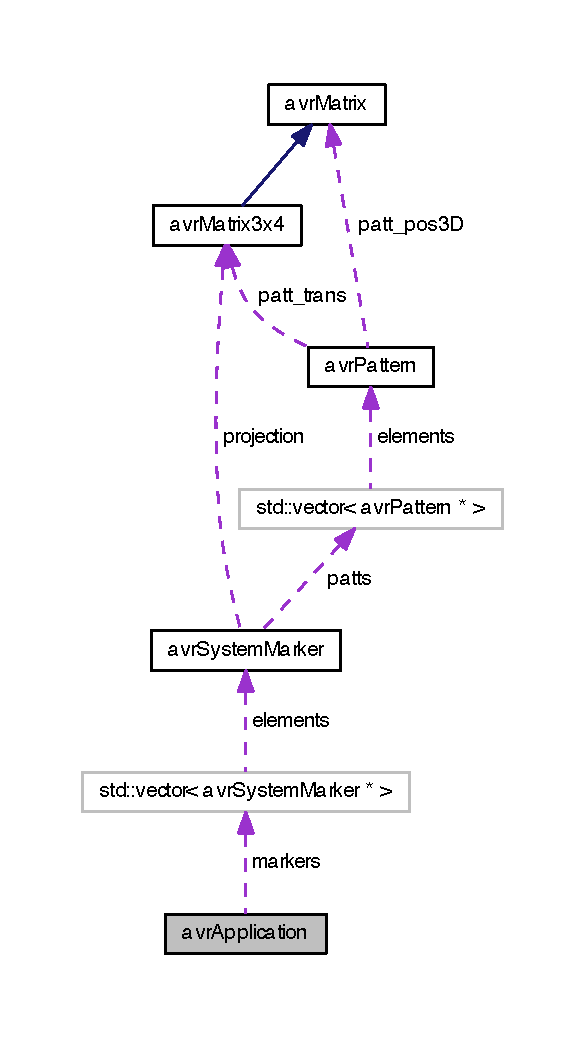
\includegraphics[width=281pt]{classavr_application__coll__graph}
\end{center}
\end{figure}
\subsection*{Public Member Functions}
\begin{DoxyCompactItemize}
\item 
\hypertarget{classavr_application_adbbf1bd55fd50ee3056d72a37800fd01}{void \hyperlink{classavr_application_adbbf1bd55fd50ee3056d72a37800fd01}{set\-New\-System} (\hyperlink{classavr_system_marker}{avr\-System\-Marker} $\ast$new\-System)}\label{classavr_application_adbbf1bd55fd50ee3056d72a37800fd01}

\begin{DoxyCompactList}\small\item\em sets a new markers system \end{DoxyCompactList}\item 
\hypertarget{classavr_application_a107ebe731d1d60bff93c1c54b66c5791}{\hyperlink{classavr_system_marker}{avr\-System\-Marker} $\ast$ \hyperlink{classavr_application_a107ebe731d1d60bff93c1c54b66c5791}{get\-System} (int index=0)}\label{classavr_application_a107ebe731d1d60bff93c1c54b66c5791}

\begin{DoxyCompactList}\small\item\em gets a markers system (default is first system) \end{DoxyCompactList}\item 
\hypertarget{classavr_application_a8f042f746899835204930bff38ad8ecd}{\hyperlink{classavr_pattern}{avr\-Pattern} \hyperlink{classavr_application_a8f042f746899835204930bff38ad8ecd}{get\-Pattern} (int index=0)}\label{classavr_application_a8f042f746899835204930bff38ad8ecd}

\begin{DoxyCompactList}\small\item\em gets a marker pattern (default is firts pattern of the first system) \end{DoxyCompactList}\item 
\hypertarget{classavr_application_a6bb369dd9daf3ad30d5aad4808bdcd06}{int \hyperlink{classavr_application_a6bb369dd9daf3ad30d5aad4808bdcd06}{number\-Patts} ()}\label{classavr_application_a6bb369dd9daf3ad30d5aad4808bdcd06}

\begin{DoxyCompactList}\small\item\em returns the total number marker patterns of the application \end{DoxyCompactList}\item 
\hypertarget{classavr_application_a6d101b2dd2ec280cea6e4110dfcfabe3}{void \hyperlink{classavr_application_a6d101b2dd2ec280cea6e4110dfcfabe3}{set\-Main\-Video\-Output} (unsigned int xwin, unsigned int ywin)}\label{classavr_application_a6d101b2dd2ec280cea6e4110dfcfabe3}

\begin{DoxyCompactList}\small\item\em says in which window the main video will be displayed \end{DoxyCompactList}\item 
\hypertarget{classavr_application_a8be1c8718562df698a25ec7474e861fa}{void \hyperlink{classavr_application_a8be1c8718562df698a25ec7474e861fa}{enable\-Mode\-Threshold} (unsigned int xwin=0, unsigned int ywin=0)}\label{classavr_application_a8be1c8718562df698a25ec7474e861fa}

\begin{DoxyCompactList}\small\item\em enable threshold image visualization (by default in main video output) \end{DoxyCompactList}\item 
\hypertarget{classavr_application_ad2097ba1b941d67a1225d8cb9201239c}{void \hyperlink{classavr_application_ad2097ba1b941d67a1225d8cb9201239c}{disable\-Mode\-Threshold} ()}\label{classavr_application_ad2097ba1b941d67a1225d8cb9201239c}

\begin{DoxyCompactList}\small\item\em disable threshold image visualization \end{DoxyCompactList}\item 
\hypertarget{classavr_application_a4775aac0f1c623a5a54d6a24518ab2bc}{bool \hyperlink{classavr_application_a4775aac0f1c623a5a54d6a24518ab2bc}{is\-Threshold\-Mode} ()}\label{classavr_application_a4775aac0f1c623a5a54d6a24518ab2bc}

\begin{DoxyCompactList}\small\item\em checks if threshold image visualization is enabled or disabled \end{DoxyCompactList}\item 
\hypertarget{classavr_application_abb48275b9f81a7acbe6a64caa143905b}{int \hyperlink{classavr_application_abb48275b9f81a7acbe6a64caa143905b}{get\-Thresh\-Hold} ()}\label{classavr_application_abb48275b9f81a7acbe6a64caa143905b}

\begin{DoxyCompactList}\small\item\em gets theshold value \end{DoxyCompactList}\item 
\hypertarget{classavr_application_a7f8fbffc3401662d4a9505396240203f}{double \hyperlink{classavr_application_a7f8fbffc3401662d4a9505396240203f}{get\-Frame\-Rate} ()}\label{classavr_application_a7f8fbffc3401662d4a9505396240203f}

\begin{DoxyCompactList}\small\item\em gets frame rate value \end{DoxyCompactList}\item 
\hypertarget{classavr_application_a554301792a3e5fc1b94a91a61f06c776}{void \hyperlink{classavr_application_a554301792a3e5fc1b94a91a61f06c776}{reset\-Frame\-Rate} ()}\label{classavr_application_a554301792a3e5fc1b94a91a61f06c776}

\begin{DoxyCompactList}\small\item\em restarts counting frames \end{DoxyCompactList}\item 
\hypertarget{classavr_application_a1a8ccf19884216cd20551209a8e2f467}{void \hyperlink{classavr_application_a1a8ccf19884216cd20551209a8e2f467}{render\-Context2\-D} ()}\label{classavr_application_a1a8ccf19884216cd20551209a8e2f467}

\begin{DoxyCompactList}\small\item\em changes the context renderization for 2\-D \end{DoxyCompactList}\item 
\hypertarget{classavr_application_a1877b70f4c21aef658da5b5d89949240}{void \hyperlink{classavr_application_a1877b70f4c21aef658da5b5d89949240}{render\-Context3\-D} (unsigned int xwin=0, unsigned int ywin=0)}\label{classavr_application_a1877b70f4c21aef658da5b5d89949240}

\begin{DoxyCompactList}\small\item\em changes the context renderization for 3\-D and sets video output (by default in main video output) \end{DoxyCompactList}\item 
\hypertarget{classavr_application_aee3a9519894f816f0629d6f7781427df}{void \hyperlink{classavr_application_aee3a9519894f816f0629d6f7781427df}{set\-Camera\-Files} ()}\label{classavr_application_aee3a9519894f816f0629d6f7781427df}

\begin{DoxyCompactList}\small\item\em sets default camera files \end{DoxyCompactList}\item 
\hypertarget{classavr_application_a398f541cc785cbedeaf18ff240d633a8}{void \hyperlink{classavr_application_a398f541cc785cbedeaf18ff240d633a8}{set\-Threshold} ()}\label{classavr_application_a398f541cc785cbedeaf18ff240d633a8}

\begin{DoxyCompactList}\small\item\em sets default threshold value (is 100) \end{DoxyCompactList}\item 
\hypertarget{classavr_application_a0b3fcb128e6ce2903905f9d595c32990}{void \hyperlink{classavr_application_a0b3fcb128e6ce2903905f9d595c32990}{add\-Pattern} (const char $\ast$filename, double patt\-\_\-width, double $\ast$patt\-\_\-center=N\-U\-L\-L, void($\ast$draw\-Function)(void)=N\-U\-L\-L)}\label{classavr_application_a0b3fcb128e6ce2903905f9d595c32990}

\begin{DoxyCompactList}\small\item\em creates a new \char`\"{}\-Single markers system\char`\"{} and registers a new marker pattern in this system (secondary display callback) \end{DoxyCompactList}\item 
\hypertarget{classavr_application_abbb6e9ba0158310dc26916a5838e91f8}{void \hyperlink{classavr_application_abbb6e9ba0158310dc26916a5838e91f8}{add\-Pattern} (const char $\ast$filename, double patt\-\_\-width, double $\ast$patt\-\_\-center=N\-U\-L\-L, void($\ast$draw\-Function)(int)=N\-U\-L\-L)}\label{classavr_application_abbb6e9ba0158310dc26916a5838e91f8}

\begin{DoxyCompactList}\small\item\em creates a new \char`\"{}\-Single markers system\char`\"{} and registers a new marker pattern in this system (main display callback) \end{DoxyCompactList}\item 
\hypertarget{classavr_application_a43b5fec0a9d6f3aca838d65101d3fe70}{void \hyperlink{classavr_application_a43b5fec0a9d6f3aca838d65101d3fe70}{add\-Patterns} (const char $\ast$filename, int holder\-Mode, void($\ast$draw\-Function)(void)=N\-U\-L\-L)}\label{classavr_application_a43b5fec0a9d6f3aca838d65101d3fe70}

\begin{DoxyCompactList}\small\item\em creates a new \char`\"{}\-Auto\-Multi markers system\char`\"{} and registers the new markers patterns in this system (secondary display callback) \end{DoxyCompactList}\item 
\hypertarget{classavr_application_a079003c61990d363c64dd2b9eab10739}{void \hyperlink{classavr_application_a079003c61990d363c64dd2b9eab10739}{add\-Patterns} (const char $\ast$filename, int holder\-Mode, void($\ast$draw\-Function)(int)=N\-U\-L\-L)}\label{classavr_application_a079003c61990d363c64dd2b9eab10739}

\begin{DoxyCompactList}\small\item\em creates a new \char`\"{}\-Auto\-Multi markers system\char`\"{} and registers the new markers patterns in this system (main display callback) \end{DoxyCompactList}\item 
\hypertarget{classavr_application_a854b6dc36d8e647ffd07ac5ecd4e9a11}{void \hyperlink{classavr_application_a854b6dc36d8e647ffd07ac5ecd4e9a11}{add\-Patterns} (const char $\ast$filename, void($\ast$draw\-Function)(void)=N\-U\-L\-L)}\label{classavr_application_a854b6dc36d8e647ffd07ac5ecd4e9a11}

\begin{DoxyCompactList}\small\item\em creates a new \char`\"{}\-Multi markers system\char`\"{} and registers the new markers patterns in this system (secondary display callback) \end{DoxyCompactList}\item 
\hypertarget{classavr_application_afb26356f31325140cbf623d08cdbc90b}{void \hyperlink{classavr_application_afb26356f31325140cbf623d08cdbc90b}{add\-Patterns} (const char $\ast$filename, void($\ast$draw\-Function)(int)=N\-U\-L\-L)}\label{classavr_application_afb26356f31325140cbf623d08cdbc90b}

\begin{DoxyCompactList}\small\item\em creates a new \char`\"{}\-Auto\-Multi markers system\char`\"{} and registers the new markers patterns in this system (main display callback) \end{DoxyCompactList}\item 
\hypertarget{classavr_application_a2bfb6a28314fd0e9207d1d50c245313b}{void \hyperlink{classavr_application_a2bfb6a28314fd0e9207d1d50c245313b}{set\-Threshold} (int thresh)}\label{classavr_application_a2bfb6a28314fd0e9207d1d50c245313b}

\begin{DoxyCompactList}\small\item\em sets a new threshold value \end{DoxyCompactList}\item 
void \hyperlink{classavr_application_a27c801a3483c796d7987eca14444fc22}{set\-Camera\-Files} (char $\ast$vconf, char $\ast$cparam\-\_\-name, int xwin=0, int ywin=0)
\begin{DoxyCompactList}\small\item\em sets the camera files and defines the number of video outputs (by default only the main video output) \end{DoxyCompactList}\item 
\hypertarget{classavr_application_a1c22de4137bf8f3d898265b0989ede8e}{void \hyperlink{classavr_application_a1c22de4137bf8f3d898265b0989ede8e}{set\-Reshape\-Callback} (void($\ast$reshape\-Function)(int w, int h))}\label{classavr_application_a1c22de4137bf8f3d898265b0989ede8e}

\begin{DoxyCompactList}\small\item\em sets reshape callback \end{DoxyCompactList}\item 
\hypertarget{classavr_application_a8f3ad5c74ee7e337e87f6f78baf93141}{void \hyperlink{classavr_application_a8f3ad5c74ee7e337e87f6f78baf93141}{set\-Visibility\-Callback} (void($\ast$visibility\-Function)(int visible))}\label{classavr_application_a8f3ad5c74ee7e337e87f6f78baf93141}

\begin{DoxyCompactList}\small\item\em sets visibility callback \end{DoxyCompactList}\item 
\hypertarget{classavr_application_a9513e1755d955acc17cbbf5fcd331a07}{void \hyperlink{classavr_application_a9513e1755d955acc17cbbf5fcd331a07}{set\-Special\-Callback} (void($\ast$special\-Function)(int key, int x, int y))}\label{classavr_application_a9513e1755d955acc17cbbf5fcd331a07}

\begin{DoxyCompactList}\small\item\em sets special keyboard events callback \end{DoxyCompactList}\item 
\hypertarget{classavr_application_aa957ba4d970f15984767eeadb42ffafa}{void \hyperlink{classavr_application_aa957ba4d970f15984767eeadb42ffafa}{set\-Key\-Callback} (void($\ast$key\-Event)(unsigned char key, int x, int y))}\label{classavr_application_aa957ba4d970f15984767eeadb42ffafa}

\begin{DoxyCompactList}\small\item\em sets keyboard events callback \end{DoxyCompactList}\item 
\hypertarget{classavr_application_ac09ee787d3e0baafd373967a29c70f22}{void \hyperlink{classavr_application_ac09ee787d3e0baafd373967a29c70f22}{set\-Motion\-Callback} (void($\ast$motion\-Event)(int x, int y))}\label{classavr_application_ac09ee787d3e0baafd373967a29c70f22}

\begin{DoxyCompactList}\small\item\em sets motion events callback \end{DoxyCompactList}\item 
\hypertarget{classavr_application_af7c0e85b3ea4c60692698f25daa5980e}{void \hyperlink{classavr_application_af7c0e85b3ea4c60692698f25daa5980e}{set\-Mouse\-Callback} (void($\ast$mouse\-Event)(int button, int state, int x, int y))}\label{classavr_application_af7c0e85b3ea4c60692698f25daa5980e}

\begin{DoxyCompactList}\small\item\em sets mouse events callback \end{DoxyCompactList}\item 
\hypertarget{classavr_application_a582980be4415041999d879ddc79cd326}{void \hyperlink{classavr_application_a582980be4415041999d879ddc79cd326}{main\-Loop} ()}\label{classavr_application_a582980be4415041999d879ddc79cd326}

\begin{DoxyCompactList}\small\item\em main loop application \end{DoxyCompactList}\item 
\hypertarget{classavr_application_ac9ca425be51b316bba545440a8c0db1c}{void \hyperlink{classavr_application_ac9ca425be51b316bba545440a8c0db1c}{start} ()}\label{classavr_application_ac9ca425be51b316bba545440a8c0db1c}

\begin{DoxyCompactList}\small\item\em Starts main loop application (called after sets the files, patterns and callbacks for start application) \end{DoxyCompactList}\item 
\hypertarget{classavr_application_a5fad6efc429d79c8e956833e03eda670}{void \hyperlink{classavr_application_a5fad6efc429d79c8e956833e03eda670}{stop} ()}\label{classavr_application_a5fad6efc429d79c8e956833e03eda670}

\begin{DoxyCompactList}\small\item\em Stops video captures and exit application (called in the end of the applications) \end{DoxyCompactList}\item 
void \hyperlink{classavr_application_a3132d9cf3eeb1eb75988c3e99f9aabe4}{set\-Project\-Info} (std\-::string project\-Name, std\-::string authors, std\-::string info, std\-::string required\-Markers)
\begin{DoxyCompactList}\small\item\em sets project informations (optional) \end{DoxyCompactList}\item 
\hypertarget{classavr_application_a1a2c0c94b3251b39e478b769cf3abaca}{void \hyperlink{classavr_application_a1a2c0c94b3251b39e478b769cf3abaca}{print\-Project\-Info} ()}\label{classavr_application_a1a2c0c94b3251b39e478b769cf3abaca}

\begin{DoxyCompactList}\small\item\em shows project information in the terminal \end{DoxyCompactList}\end{DoxyCompactItemize}
\subsection*{Protected Attributes}
\begin{DoxyCompactItemize}
\item 
\hypertarget{classavr_application_aca46c12fb13329b90f4b20c34547e30b}{std\-::vector$<$ \hyperlink{classavr_system_marker}{avr\-System\-Marker} $\ast$ $>$ \hyperlink{classavr_application_aca46c12fb13329b90f4b20c34547e30b}{markers}}\label{classavr_application_aca46c12fb13329b90f4b20c34547e30b}

\begin{DoxyCompactList}\small\item\em vector with the markers systems that aggregate the application \end{DoxyCompactList}\end{DoxyCompactItemize}


\subsection{Detailed Description}
main class of the applications 

This class is a states machine. Controls the entire execution flow of the application. Manages all markers systems, the outputs and properties video and makes calls for the callbacks. 

\subsection{Member Function Documentation}
\hypertarget{classavr_application_a27c801a3483c796d7987eca14444fc22}{\index{avr\-Application@{avr\-Application}!set\-Camera\-Files@{set\-Camera\-Files}}
\index{set\-Camera\-Files@{set\-Camera\-Files}!avrApplication@{avr\-Application}}
\subsubsection[{set\-Camera\-Files}]{\setlength{\rightskip}{0pt plus 5cm}void avr\-Application\-::set\-Camera\-Files (
\begin{DoxyParamCaption}
\item[{char $\ast$}]{vconf, }
\item[{char $\ast$}]{cparam\-\_\-name, }
\item[{int}]{xwin = {\ttfamily 0}, }
\item[{int}]{ywin = {\ttfamily 0}}
\end{DoxyParamCaption}
)}}\label{classavr_application_a27c801a3483c796d7987eca14444fc22}


sets the camera files and defines the number of video outputs (by default only the main video output) 

This function inicializes the camera configuration and the intrinsics parameters of the camera. At end, the window is created. 
\begin{DoxyParams}{Parameters}
{\em vconf} & camera configuration path file \\
\hline
{\em cparam\-\_\-name} & path with intrinsics parameters file of the camera \\
\hline
{\em xwin} & default is 0 \\
\hline
{\em ywin} & default is 0 \\
\hline
\end{DoxyParams}
\begin{DoxyReturn}{Returns}
void 
\end{DoxyReturn}
\hypertarget{classavr_application_a3132d9cf3eeb1eb75988c3e99f9aabe4}{\index{avr\-Application@{avr\-Application}!set\-Project\-Info@{set\-Project\-Info}}
\index{set\-Project\-Info@{set\-Project\-Info}!avrApplication@{avr\-Application}}
\subsubsection[{set\-Project\-Info}]{\setlength{\rightskip}{0pt plus 5cm}void avr\-Application\-::set\-Project\-Info (
\begin{DoxyParamCaption}
\item[{std\-::string}]{project\-Name, }
\item[{std\-::string}]{authors, }
\item[{std\-::string}]{info, }
\item[{std\-::string}]{required\-Markers}
\end{DoxyParamCaption}
)}}\label{classavr_application_a3132d9cf3eeb1eb75988c3e99f9aabe4}


sets project informations (optional) 


\begin{DoxyParams}{Parameters}
{\em project\-Name} & application name \\
\hline
{\em authors} & authors names of application \\
\hline
{\em info} & more informations \\
\hline
{\em required\-Markers} & required markers by application \\
\hline
\end{DoxyParams}
\begin{DoxyReturn}{Returns}
void 
\end{DoxyReturn}


The documentation for this class was generated from the following file\-:\begin{DoxyCompactItemize}
\item 
avr\-Application.\-h\end{DoxyCompactItemize}

\hypertarget{classavr_matrix}{\section{avr\-Matrix Class Reference}
\label{classavr_matrix}\index{avr\-Matrix@{avr\-Matrix}}
}


represents a nxm dimension matrix  




{\ttfamily \#include \char`\"{}avr\-Matrix.\-h\char`\"{}}



Inheritance diagram for avr\-Matrix\-:\nopagebreak
\begin{figure}[H]
\begin{center}
\leavevmode
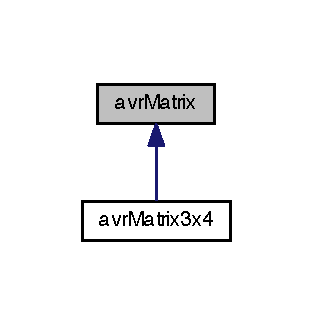
\includegraphics[width=150pt]{classavr_matrix__inherit__graph}
\end{center}
\end{figure}
\subsection*{Public Member Functions}
\begin{DoxyCompactItemize}
\item 
\hypertarget{classavr_matrix_a46991bd48c86dae9b1d8a987381e1401}{{\bfseries avr\-Matrix} (int \hyperlink{classavr_matrix_a3e27175e91c4565f66ec6e590fc86520}{row}, int clm)}\label{classavr_matrix_a46991bd48c86dae9b1d8a987381e1401}

\item 
\hypertarget{classavr_matrix_ad3ab687c2493bf5729923091794b6a58}{\hyperlink{classavr_matrix}{avr\-Matrix} \& \hyperlink{classavr_matrix_ad3ab687c2493bf5729923091794b6a58}{operator=} (const \hyperlink{classavr_matrix}{avr\-Matrix} \&)}\label{classavr_matrix_ad3ab687c2493bf5729923091794b6a58}

\begin{DoxyCompactList}\small\item\em copy constructor \end{DoxyCompactList}\item 
\hyperlink{classavr_matrix}{avr\-Matrix} \& \hyperlink{classavr_matrix_ab0a3eb564d518e9bb19423e38225d5ab}{operator+} (const \hyperlink{classavr_matrix}{avr\-Matrix} \&)  throw (std\-::invalid\-\_\-argument\&)
\begin{DoxyCompactList}\small\item\em sum two matrices (this object + parameter matrix) \end{DoxyCompactList}\item 
\hyperlink{classavr_matrix}{avr\-Matrix} \& \hyperlink{classavr_matrix_a158008cbe2eca3d0b7eae73354b8e85a}{operator-\/} (const \hyperlink{classavr_matrix}{avr\-Matrix} \&)  throw (std\-::invalid\-\_\-argument\&)
\begin{DoxyCompactList}\small\item\em subtracts two matrices (this object -\/ parameter matrix) \end{DoxyCompactList}\item 
\hyperlink{classavr_matrix}{avr\-Matrix} \& \hyperlink{classavr_matrix_a005b285625ae8e9c677cde1c42309c71}{operator$\ast$} (const \hyperlink{classavr_matrix}{avr\-Matrix} \&)  throw (std\-::invalid\-\_\-argument\&)
\begin{DoxyCompactList}\small\item\em multiplies two matrices (this object x parameter matrix) \end{DoxyCompactList}\item 
\hyperlink{classavr_matrix}{avr\-Matrix} \& \hyperlink{classavr_matrix_a90beb569a126464ac64d17a3a86d2b32}{operator$\ast$} (double scalar)
\begin{DoxyCompactList}\small\item\em multiplies the matrix by a scalar number (this object x scalar number) \end{DoxyCompactList}\item 
\hyperlink{classavr_matrix}{avr\-Matrix} \& \hyperlink{classavr_matrix_a5513ce11445f37491ae0aff012959498}{inverse} () const   throw (std\-::domain\-\_\-error\&)
\begin{DoxyCompactList}\small\item\em calculates the inverse matrix \end{DoxyCompactList}\item 
\hyperlink{classavr_matrix}{avr\-Matrix} \& \hyperlink{classavr_matrix_ac7e10b075dfcc8a35ef001cb053580d0}{trasposed} () const 
\begin{DoxyCompactList}\small\item\em calculates the transposed matrix \end{DoxyCompactList}\item 
double \hyperlink{classavr_matrix_a778cdf2fd6644178cc0d43a6c9ff439c}{determinant} () const 
\begin{DoxyCompactList}\small\item\em calculates the determinant of the matrix \end{DoxyCompactList}\item 
virtual void \hyperlink{classavr_matrix_a242c461dc5189ba5ea51d7de92b50eea}{add} (double element, int \hyperlink{classavr_matrix_a3e27175e91c4565f66ec6e590fc86520}{row}, int clm)  throw (std\-::out\-\_\-of\-\_\-range\&)
\begin{DoxyCompactList}\small\item\em adds a new element in matrix \end{DoxyCompactList}\item 
virtual double \hyperlink{classavr_matrix_a24e5e23cfcba9774ce4a10d8a027b622}{access} (int \hyperlink{classavr_matrix_a3e27175e91c4565f66ec6e590fc86520}{row}, int clm) const   throw (std\-::out\-\_\-of\-\_\-range\&)
\begin{DoxyCompactList}\small\item\em access an element in matrix \end{DoxyCompactList}\item 
virtual void \hyperlink{classavr_matrix_a28dd43731f25153dff0a121004f23d34}{print} (std\-::string name=\char`\"{}\char`\"{}, int decimals=5) const 
\begin{DoxyCompactList}\small\item\em shows a matrix \end{DoxyCompactList}\item 
\hypertarget{classavr_matrix_a3e27175e91c4565f66ec6e590fc86520}{virtual int \hyperlink{classavr_matrix_a3e27175e91c4565f66ec6e590fc86520}{row} () const }\label{classavr_matrix_a3e27175e91c4565f66ec6e590fc86520}

\begin{DoxyCompactList}\small\item\em Get row dimension. \end{DoxyCompactList}\item 
\hypertarget{classavr_matrix_a87a5d5fee3d3f8ff1970d077eee52ce5}{virtual int \hyperlink{classavr_matrix_a87a5d5fee3d3f8ff1970d077eee52ce5}{column} () const }\label{classavr_matrix_a87a5d5fee3d3f8ff1970d077eee52ce5}

\begin{DoxyCompactList}\small\item\em Get column dimension. \end{DoxyCompactList}\item 
virtual double $\ast$$\ast$ \hyperlink{classavr_matrix_af06d1669ec6c8f2be5e2d2cf421e1dcd}{matrix} () const 
\begin{DoxyCompactList}\small\item\em Get matrix in c format. \end{DoxyCompactList}\item 
\hypertarget{classavr_matrix_a309f5af755f83a47327e6e88034d0680}{void \hyperlink{classavr_matrix_a309f5af755f83a47327e6e88034d0680}{set\-Identity\-Matrix} ()}\label{classavr_matrix_a309f5af755f83a47327e6e88034d0680}

\begin{DoxyCompactList}\small\item\em initialize matrix with identity matrix \end{DoxyCompactList}\end{DoxyCompactItemize}
\subsection*{Protected Attributes}
\begin{DoxyCompactItemize}
\item 
\hypertarget{classavr_matrix_acc47cfe71e4829cae8a64b29c15463da}{double $\ast$ \hyperlink{classavr_matrix_acc47cfe71e4829cae8a64b29c15463da}{matrixx}}\label{classavr_matrix_acc47cfe71e4829cae8a64b29c15463da}

\begin{DoxyCompactList}\small\item\em array which store elements (position = i $\ast$ clms + j) \end{DoxyCompactList}\end{DoxyCompactItemize}


\subsection{Detailed Description}
represents a nxm dimension matrix 

This class simplifies the operations between nxm dimension matrices 
\begin{DoxyParams}{Parameters}
{\em row} & Row dimension \\
\hline
{\em clm} & Column dimension \\
\hline
\end{DoxyParams}


\subsection{Member Function Documentation}
\hypertarget{classavr_matrix_a24e5e23cfcba9774ce4a10d8a027b622}{\index{avr\-Matrix@{avr\-Matrix}!access@{access}}
\index{access@{access}!avrMatrix@{avr\-Matrix}}
\subsubsection[{access}]{\setlength{\rightskip}{0pt plus 5cm}virtual double avr\-Matrix\-::access (
\begin{DoxyParamCaption}
\item[{int}]{row, }
\item[{int}]{clm}
\end{DoxyParamCaption}
) const throw  std\-::out\-\_\-of\-\_\-range \&) \hspace{0.3cm}{\ttfamily [virtual]}}}\label{classavr_matrix_a24e5e23cfcba9774ce4a10d8a027b622}


access an element in matrix 


\begin{DoxyParams}[1]{Parameters}
\mbox{\tt in}  & {\em row} & index of row \\
\hline
\mbox{\tt in}  & {\em clm} & index of column \\
\hline
\end{DoxyParams}
\begin{DoxyReturn}{Returns}
double element of the position \mbox{[}row\mbox{]}\mbox{[}clm\mbox{]} 
\end{DoxyReturn}

\begin{DoxyExceptions}{Exceptions}
{\em out\-\_\-of\-\_\-range\&} & if invalid indexes \\
\hline
\end{DoxyExceptions}


Reimplemented in \hyperlink{classavr_matrix3x4_a7782b5c0211411a41e5293b038974ff1}{avr\-Matrix3x4}.

\hypertarget{classavr_matrix_a242c461dc5189ba5ea51d7de92b50eea}{\index{avr\-Matrix@{avr\-Matrix}!add@{add}}
\index{add@{add}!avrMatrix@{avr\-Matrix}}
\subsubsection[{add}]{\setlength{\rightskip}{0pt plus 5cm}virtual void avr\-Matrix\-::add (
\begin{DoxyParamCaption}
\item[{double}]{element, }
\item[{int}]{row, }
\item[{int}]{clm}
\end{DoxyParamCaption}
) throw  std\-::out\-\_\-of\-\_\-range \&) \hspace{0.3cm}{\ttfamily [virtual]}}}\label{classavr_matrix_a242c461dc5189ba5ea51d7de92b50eea}


adds a new element in matrix 


\begin{DoxyParams}[1]{Parameters}
\mbox{\tt in}  & {\em element} & new element to add \\
\hline
\mbox{\tt in}  & {\em row} & index of row \\
\hline
\mbox{\tt in}  & {\em clm} & index of column \\
\hline
\end{DoxyParams}
\begin{DoxyReturn}{Returns}
void 
\end{DoxyReturn}

\begin{DoxyExceptions}{Exceptions}
{\em out\-\_\-of\-\_\-range\&} & if invalid indexes \\
\hline
\end{DoxyExceptions}


Reimplemented in \hyperlink{classavr_matrix3x4_a4e47d85232a5abe1ccc8cd0ba72e4e18}{avr\-Matrix3x4}.

\hypertarget{classavr_matrix_a778cdf2fd6644178cc0d43a6c9ff439c}{\index{avr\-Matrix@{avr\-Matrix}!determinant@{determinant}}
\index{determinant@{determinant}!avrMatrix@{avr\-Matrix}}
\subsubsection[{determinant}]{\setlength{\rightskip}{0pt plus 5cm}double avr\-Matrix\-::determinant (
\begin{DoxyParamCaption}
{}
\end{DoxyParamCaption}
) const}}\label{classavr_matrix_a778cdf2fd6644178cc0d43a6c9ff439c}


calculates the determinant of the matrix 

\begin{DoxyNote}{Note}
if the non-\/square matrix, determinant equals to zero
\end{DoxyNote}
\begin{DoxyReturn}{Returns}
double determinant value 
\end{DoxyReturn}
\hypertarget{classavr_matrix_a5513ce11445f37491ae0aff012959498}{\index{avr\-Matrix@{avr\-Matrix}!inverse@{inverse}}
\index{inverse@{inverse}!avrMatrix@{avr\-Matrix}}
\subsubsection[{inverse}]{\setlength{\rightskip}{0pt plus 5cm}{\bf avr\-Matrix}\& avr\-Matrix\-::inverse (
\begin{DoxyParamCaption}
{}
\end{DoxyParamCaption}
) const throw  std\-::domain\-\_\-error \&) }}\label{classavr_matrix_a5513ce11445f37491ae0aff012959498}


calculates the inverse matrix 

\begin{DoxyReturn}{Returns}
\hyperlink{classavr_matrix}{avr\-Matrix}\& inverse matrix 
\end{DoxyReturn}

\begin{DoxyExceptions}{Exceptions}
{\em domain\-\_\-error\&} & not exists the inverse \\
\hline
\end{DoxyExceptions}
\hypertarget{classavr_matrix_af06d1669ec6c8f2be5e2d2cf421e1dcd}{\index{avr\-Matrix@{avr\-Matrix}!matrix@{matrix}}
\index{matrix@{matrix}!avrMatrix@{avr\-Matrix}}
\subsubsection[{matrix}]{\setlength{\rightskip}{0pt plus 5cm}virtual double$\ast$$\ast$ avr\-Matrix\-::matrix (
\begin{DoxyParamCaption}
{}
\end{DoxyParamCaption}
) const\hspace{0.3cm}{\ttfamily [virtual]}}}\label{classavr_matrix_af06d1669ec6c8f2be5e2d2cf421e1dcd}


Get matrix in c format. 

The reference is for a new matrix, not for the attribute 'matrixx' \begin{DoxyReturn}{Returns}
double$\ast$$\ast$ matrix in c format (mat\mbox{[}n\mbox{]}\mbox{[}m\mbox{]}) 
\end{DoxyReturn}


Reimplemented in \hyperlink{classavr_matrix3x4_ab51a103b8c059a18324d4c675a47a0fa}{avr\-Matrix3x4}.

\hypertarget{classavr_matrix_a005b285625ae8e9c677cde1c42309c71}{\index{avr\-Matrix@{avr\-Matrix}!operator$\ast$@{operator$\ast$}}
\index{operator$\ast$@{operator$\ast$}!avrMatrix@{avr\-Matrix}}
\subsubsection[{operator$\ast$}]{\setlength{\rightskip}{0pt plus 5cm}{\bf avr\-Matrix}\& avr\-Matrix\-::operator$\ast$ (
\begin{DoxyParamCaption}
\item[{const {\bf avr\-Matrix} \&}]{}
\end{DoxyParamCaption}
) throw  std\-::invalid\-\_\-argument \&) }}\label{classavr_matrix_a005b285625ae8e9c677cde1c42309c71}


multiplies two matrices (this object x parameter matrix) 

\begin{DoxyPrecond}{Precondition}
column dimension of this object must be equal the row dimension of parameter matrix
\end{DoxyPrecond}

\begin{DoxyParams}[1]{Parameters}
\mbox{\tt in}  & {\em avr\-Matrix\&} & \\
\hline
\end{DoxyParams}
\begin{DoxyReturn}{Returns}
\hyperlink{classavr_matrix}{avr\-Matrix}\& result matrix 
\end{DoxyReturn}

\begin{DoxyExceptions}{Exceptions}
{\em invalid\-\_\-argument\&} & if pre-\/condition doesn't satisfied \\
\hline
\end{DoxyExceptions}
\hypertarget{classavr_matrix_a90beb569a126464ac64d17a3a86d2b32}{\index{avr\-Matrix@{avr\-Matrix}!operator$\ast$@{operator$\ast$}}
\index{operator$\ast$@{operator$\ast$}!avrMatrix@{avr\-Matrix}}
\subsubsection[{operator$\ast$}]{\setlength{\rightskip}{0pt plus 5cm}{\bf avr\-Matrix}\& avr\-Matrix\-::operator$\ast$ (
\begin{DoxyParamCaption}
\item[{double}]{scalar}
\end{DoxyParamCaption}
)}}\label{classavr_matrix_a90beb569a126464ac64d17a3a86d2b32}


multiplies the matrix by a scalar number (this object x scalar number) 


\begin{DoxyParams}[1]{Parameters}
\mbox{\tt in}  & {\em scalar} & scalar value \\
\hline
\end{DoxyParams}
\begin{DoxyReturn}{Returns}
\hyperlink{classavr_matrix}{avr\-Matrix}\& result matrix 
\end{DoxyReturn}
\hypertarget{classavr_matrix_ab0a3eb564d518e9bb19423e38225d5ab}{\index{avr\-Matrix@{avr\-Matrix}!operator+@{operator+}}
\index{operator+@{operator+}!avrMatrix@{avr\-Matrix}}
\subsubsection[{operator+}]{\setlength{\rightskip}{0pt plus 5cm}{\bf avr\-Matrix}\& avr\-Matrix\-::operator+ (
\begin{DoxyParamCaption}
\item[{const {\bf avr\-Matrix} \&}]{}
\end{DoxyParamCaption}
) throw  std\-::invalid\-\_\-argument \&) }}\label{classavr_matrix_ab0a3eb564d518e9bb19423e38225d5ab}


sum two matrices (this object + parameter matrix) 

\begin{DoxyPrecond}{Precondition}
dimension of the matrices must be equal
\end{DoxyPrecond}

\begin{DoxyParams}[1]{Parameters}
\mbox{\tt in}  & {\em avr\-Matrix\&} & \\
\hline
\end{DoxyParams}
\begin{DoxyReturn}{Returns}
\hyperlink{classavr_matrix}{avr\-Matrix}\& result matrix 
\end{DoxyReturn}

\begin{DoxyExceptions}{Exceptions}
{\em invalid\-\_\-argument\&} & if pre-\/condition doesn't satisfied \\
\hline
\end{DoxyExceptions}
\hypertarget{classavr_matrix_a158008cbe2eca3d0b7eae73354b8e85a}{\index{avr\-Matrix@{avr\-Matrix}!operator-\/@{operator-\/}}
\index{operator-\/@{operator-\/}!avrMatrix@{avr\-Matrix}}
\subsubsection[{operator-\/}]{\setlength{\rightskip}{0pt plus 5cm}{\bf avr\-Matrix}\& avr\-Matrix\-::operator-\/ (
\begin{DoxyParamCaption}
\item[{const {\bf avr\-Matrix} \&}]{}
\end{DoxyParamCaption}
) throw  std\-::invalid\-\_\-argument \&) }}\label{classavr_matrix_a158008cbe2eca3d0b7eae73354b8e85a}


subtracts two matrices (this object -\/ parameter matrix) 

\begin{DoxyPrecond}{Precondition}
dimension of the matrices must be equal
\end{DoxyPrecond}

\begin{DoxyParams}[1]{Parameters}
\mbox{\tt in}  & {\em avr\-Matrix\&} & \\
\hline
\end{DoxyParams}
\begin{DoxyReturn}{Returns}
\hyperlink{classavr_matrix}{avr\-Matrix}\& result matrix 
\end{DoxyReturn}

\begin{DoxyExceptions}{Exceptions}
{\em invalid\-\_\-argument\&} & if pre-\/condition doesn't satisfied \\
\hline
\end{DoxyExceptions}
\hypertarget{classavr_matrix_a28dd43731f25153dff0a121004f23d34}{\index{avr\-Matrix@{avr\-Matrix}!print@{print}}
\index{print@{print}!avrMatrix@{avr\-Matrix}}
\subsubsection[{print}]{\setlength{\rightskip}{0pt plus 5cm}virtual void avr\-Matrix\-::print (
\begin{DoxyParamCaption}
\item[{std\-::string}]{name = {\ttfamily \char`\"{}\char`\"{}}, }
\item[{int}]{decimals = {\ttfamily 5}}
\end{DoxyParamCaption}
) const\hspace{0.3cm}{\ttfamily [virtual]}}}\label{classavr_matrix_a28dd43731f25153dff0a121004f23d34}


shows a matrix 


\begin{DoxyParams}[1]{Parameters}
\mbox{\tt in}  & {\em name} & define a name for matrix (opcional) \\
\hline
\mbox{\tt in}  & {\em decimals} & decimals number of the elements (default is 5) \\
\hline
\end{DoxyParams}
\begin{DoxyReturn}{Returns}
void 
\end{DoxyReturn}


Reimplemented in \hyperlink{classavr_matrix3x4_a5a420d32fd603ba922472c5777dbc4cb}{avr\-Matrix3x4}.

\hypertarget{classavr_matrix_ac7e10b075dfcc8a35ef001cb053580d0}{\index{avr\-Matrix@{avr\-Matrix}!trasposed@{trasposed}}
\index{trasposed@{trasposed}!avrMatrix@{avr\-Matrix}}
\subsubsection[{trasposed}]{\setlength{\rightskip}{0pt plus 5cm}{\bf avr\-Matrix}\& avr\-Matrix\-::trasposed (
\begin{DoxyParamCaption}
{}
\end{DoxyParamCaption}
) const}}\label{classavr_matrix_ac7e10b075dfcc8a35ef001cb053580d0}


calculates the transposed matrix 

\begin{DoxyReturn}{Returns}
\hyperlink{classavr_matrix}{avr\-Matrix}\& transposed matrix 
\end{DoxyReturn}


The documentation for this class was generated from the following file\-:\begin{DoxyCompactItemize}
\item 
avr\-Matrix.\-h\end{DoxyCompactItemize}

\hypertarget{classavr_matrix3x4}{\section{avr\-Matrix3x4 Class Reference}
\label{classavr_matrix3x4}\index{avr\-Matrix3x4@{avr\-Matrix3x4}}
}


represents a 3x4 dimension matrix  




{\ttfamily \#include \char`\"{}avr\-Matrix3x4.\-h\char`\"{}}



Inheritance diagram for avr\-Matrix3x4\-:\nopagebreak
\begin{figure}[H]
\begin{center}
\leavevmode
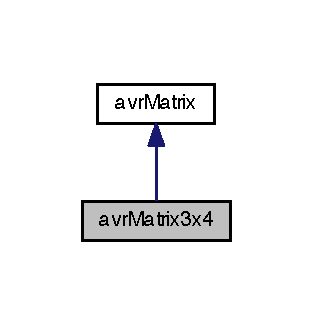
\includegraphics[width=150pt]{classavr_matrix3x4__inherit__graph}
\end{center}
\end{figure}


Collaboration diagram for avr\-Matrix3x4\-:\nopagebreak
\begin{figure}[H]
\begin{center}
\leavevmode
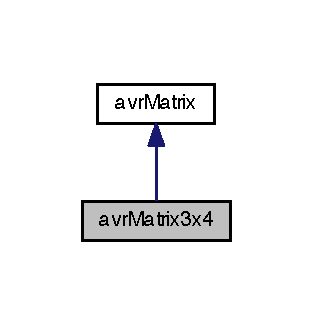
\includegraphics[width=150pt]{classavr_matrix3x4__coll__graph}
\end{center}
\end{figure}
\subsection*{Public Member Functions}
\begin{DoxyCompactItemize}
\item 
\hypertarget{classavr_matrix3x4_a36e9773d69e4fa970f8d0e20524a9aa5}{\hyperlink{classavr_matrix3x4_a36e9773d69e4fa970f8d0e20524a9aa5}{avr\-Matrix3x4} ()}\label{classavr_matrix3x4_a36e9773d69e4fa970f8d0e20524a9aa5}

\begin{DoxyCompactList}\small\item\em default constructor \end{DoxyCompactList}\item 
\hypertarget{classavr_matrix3x4_a391837f293aa73b064a41aca364d6a6b}{\hyperlink{classavr_matrix3x4_a391837f293aa73b064a41aca364d6a6b}{avr\-Matrix3x4} (const \hyperlink{classavr_matrix}{avr\-Matrix} \&)}\label{classavr_matrix3x4_a391837f293aa73b064a41aca364d6a6b}

\begin{DoxyCompactList}\small\item\em conversion constructor (if dimension \hyperlink{classavr_matrix}{avr\-Matrix} different 3x4, copy all possible elements) \end{DoxyCompactList}\item 
\hypertarget{classavr_matrix3x4_a24029bcb2ccf15bc449287bc6fbe8b26}{\hyperlink{classavr_matrix3x4_a24029bcb2ccf15bc449287bc6fbe8b26}{avr\-Matrix3x4} (double \hyperlink{classavr_matrix3x4_ab51a103b8c059a18324d4c675a47a0fa}{matrix}\mbox{[}3\mbox{]}\mbox{[}4\mbox{]})}\label{classavr_matrix3x4_a24029bcb2ccf15bc449287bc6fbe8b26}

\begin{DoxyCompactList}\small\item\em conversion constructor (from c matrix format) \end{DoxyCompactList}\item 
virtual void \hyperlink{classavr_matrix3x4_a4e47d85232a5abe1ccc8cd0ba72e4e18}{add} (double element, int \hyperlink{classavr_matrix3x4_a465a111b0339bd80a8c19418775da47f}{row}, int clm)  throw (std\-::out\-\_\-of\-\_\-range\&)
\begin{DoxyCompactList}\small\item\em adds a new element in matrix \end{DoxyCompactList}\item 
virtual double \hyperlink{classavr_matrix3x4_a7782b5c0211411a41e5293b038974ff1}{access} (int \hyperlink{classavr_matrix3x4_a465a111b0339bd80a8c19418775da47f}{row}, int clm) const   throw (std\-::out\-\_\-of\-\_\-range\&)
\begin{DoxyCompactList}\small\item\em access an element in matrix \end{DoxyCompactList}\item 
virtual void \hyperlink{classavr_matrix3x4_a5a420d32fd603ba922472c5777dbc4cb}{print} (std\-::string name=\char`\"{}\char`\"{}, int decimals=5) const 
\begin{DoxyCompactList}\small\item\em shows a matrix \end{DoxyCompactList}\item 
\hypertarget{classavr_matrix3x4_a465a111b0339bd80a8c19418775da47f}{virtual int \hyperlink{classavr_matrix3x4_a465a111b0339bd80a8c19418775da47f}{row} () const }\label{classavr_matrix3x4_a465a111b0339bd80a8c19418775da47f}

\begin{DoxyCompactList}\small\item\em returns 3 value (row dimension) \end{DoxyCompactList}\item 
\hypertarget{classavr_matrix3x4_ad5a7117cf1ded88dfb8dd01cb12aa6e9}{virtual int \hyperlink{classavr_matrix3x4_ad5a7117cf1ded88dfb8dd01cb12aa6e9}{column} () const }\label{classavr_matrix3x4_ad5a7117cf1ded88dfb8dd01cb12aa6e9}

\begin{DoxyCompactList}\small\item\em returns 4 value (column dimension) \end{DoxyCompactList}\item 
virtual double $\ast$$\ast$ \hyperlink{classavr_matrix3x4_ab51a103b8c059a18324d4c675a47a0fa}{matrix} () const 
\begin{DoxyCompactList}\small\item\em Get matrix in c format. \end{DoxyCompactList}\item 
\hypertarget{classavr_matrix3x4_a1df7a480b6c33d08d2151f513bc7541b}{\hyperlink{classavr_matrix3x4}{avr\-Matrix3x4} \& \hyperlink{classavr_matrix3x4_a1df7a480b6c33d08d2151f513bc7541b}{operator=} (const \hyperlink{classavr_matrix3x4}{avr\-Matrix3x4} \&)}\label{classavr_matrix3x4_a1df7a480b6c33d08d2151f513bc7541b}

\begin{DoxyCompactList}\small\item\em copy constructor \end{DoxyCompactList}\item 
\hyperlink{classavr_matrix3x4}{avr\-Matrix3x4} \& \hyperlink{classavr_matrix3x4_a69695710fa229029aac327a93bf67e28}{operator$\ast$} (const \hyperlink{classavr_matrix3x4}{avr\-Matrix3x4} \&)
\begin{DoxyCompactList}\small\item\em multiplies two matrices of dimension 3x4 (this object x parameter matrix) \end{DoxyCompactList}\item 
\hyperlink{classavr_matrix3x4}{avr\-Matrix3x4} \& \hyperlink{classavr_matrix3x4_af6aeaea8801d27ad4aec3c1fc9aea277}{get\-Relation\-With} (const \hyperlink{classavr_matrix3x4}{avr\-Matrix3x4} \&) const 
\begin{DoxyCompactList}\small\item\em calculates the relation matrix between the parameter matrix \end{DoxyCompactList}\item 
double \hyperlink{classavr_matrix3x4_ac05ea22d8597df4aa2b1f261ec94f8a7}{euclidian\-Distance\-Between} (const \hyperlink{classavr_matrix3x4}{avr\-Matrix3x4} \&) const 
\begin{DoxyCompactList}\small\item\em calculates the euclidian distance between the parameter matrix \end{DoxyCompactList}\item 
void \hyperlink{classavr_matrix3x4_ad03865e565b36b5e60057247216d901e}{get\-Matrix\-G\-L\-Format} (double gl\-\_\-para\mbox{[}16\mbox{]}) const 
\begin{DoxyCompactList}\small\item\em copy the elements of matrix for the matrix in Open\-G\-L format \end{DoxyCompactList}\item 
void \hyperlink{classavr_matrix3x4_a2cace74000dc095ad78c7dca07804a18}{set\-Mat\-With\-Quat\-And\-Pos} (double quat\mbox{[}4\mbox{]}, double pos\mbox{[}3\mbox{]})
\begin{DoxyCompactList}\small\item\em calculates the elements of the matrix based in the quaternion and position vectors \end{DoxyCompactList}\item 
void \hyperlink{classavr_matrix3x4_aa48c0f1da93a4aeb29750e8f2a06d968}{extract\-Quat\-And\-Pos} (double quat\mbox{[}4\mbox{]}, double pos\mbox{[}3\mbox{]}) const   throw (std\-::domain\-\_\-error\&)
\begin{DoxyCompactList}\small\item\em extracts the quaternion and position vectors of matrix \end{DoxyCompactList}\item 
\hypertarget{classavr_matrix3x4_a6af1e8d00de2afc425f86c6c9db7c45a}{double \hyperlink{classavr_matrix3x4_a6af1e8d00de2afc425f86c6c9db7c45a}{X} () const }\label{classavr_matrix3x4_a6af1e8d00de2afc425f86c6c9db7c45a}

\begin{DoxyCompactList}\small\item\em Get X position (so that access(0, 3)) \end{DoxyCompactList}\item 
\hypertarget{classavr_matrix3x4_a4fa40ec6eef8c249a3ee09191ec1f6e7}{double \hyperlink{classavr_matrix3x4_a4fa40ec6eef8c249a3ee09191ec1f6e7}{Y} () const }\label{classavr_matrix3x4_a4fa40ec6eef8c249a3ee09191ec1f6e7}

\begin{DoxyCompactList}\small\item\em Get Y position (so that access(1, 3)) \end{DoxyCompactList}\item 
\hypertarget{classavr_matrix3x4_a2ea62d9f789f86593d9e52e552775821}{double \hyperlink{classavr_matrix3x4_a2ea62d9f789f86593d9e52e552775821}{Z} () const }\label{classavr_matrix3x4_a2ea62d9f789f86593d9e52e552775821}

\begin{DoxyCompactList}\small\item\em Get Z position (so that access(2, 3)) \end{DoxyCompactList}\end{DoxyCompactItemize}
\subsection*{Additional Inherited Members}


\subsection{Detailed Description}
represents a 3x4 dimension matrix 

This class simplifies the operations between 3x4 dimension matrices and offers auxiliary functions useful in renderization routines which use transformation matrices 

\subsection{Member Function Documentation}
\hypertarget{classavr_matrix3x4_a7782b5c0211411a41e5293b038974ff1}{\index{avr\-Matrix3x4@{avr\-Matrix3x4}!access@{access}}
\index{access@{access}!avrMatrix3x4@{avr\-Matrix3x4}}
\subsubsection[{access}]{\setlength{\rightskip}{0pt plus 5cm}virtual double avr\-Matrix3x4\-::access (
\begin{DoxyParamCaption}
\item[{int}]{row, }
\item[{int}]{clm}
\end{DoxyParamCaption}
) const throw  std\-::out\-\_\-of\-\_\-range \&) \hspace{0.3cm}{\ttfamily [virtual]}}}\label{classavr_matrix3x4_a7782b5c0211411a41e5293b038974ff1}


access an element in matrix 


\begin{DoxyParams}[1]{Parameters}
\mbox{\tt in}  & {\em row} & index of row \\
\hline
\mbox{\tt in}  & {\em clm} & index of column \\
\hline
\end{DoxyParams}
\begin{DoxyReturn}{Returns}
double element of the position \mbox{[}row\mbox{]}\mbox{[}clm\mbox{]} 
\end{DoxyReturn}

\begin{DoxyExceptions}{Exceptions}
{\em out\-\_\-of\-\_\-range\&} & if invalid indexes \\
\hline
\end{DoxyExceptions}


Reimplemented from \hyperlink{classavr_matrix_a24e5e23cfcba9774ce4a10d8a027b622}{avr\-Matrix}.

\hypertarget{classavr_matrix3x4_a4e47d85232a5abe1ccc8cd0ba72e4e18}{\index{avr\-Matrix3x4@{avr\-Matrix3x4}!add@{add}}
\index{add@{add}!avrMatrix3x4@{avr\-Matrix3x4}}
\subsubsection[{add}]{\setlength{\rightskip}{0pt plus 5cm}virtual void avr\-Matrix3x4\-::add (
\begin{DoxyParamCaption}
\item[{double}]{element, }
\item[{int}]{row, }
\item[{int}]{clm}
\end{DoxyParamCaption}
) throw  std\-::out\-\_\-of\-\_\-range \&) \hspace{0.3cm}{\ttfamily [virtual]}}}\label{classavr_matrix3x4_a4e47d85232a5abe1ccc8cd0ba72e4e18}


adds a new element in matrix 


\begin{DoxyParams}[1]{Parameters}
\mbox{\tt in}  & {\em element} & new element to add \\
\hline
\mbox{\tt in}  & {\em row} & index of row \\
\hline
\mbox{\tt in}  & {\em clm} & index of column \\
\hline
\end{DoxyParams}
\begin{DoxyReturn}{Returns}
void 
\end{DoxyReturn}

\begin{DoxyExceptions}{Exceptions}
{\em out\-\_\-of\-\_\-range\&} & if invalid indexes \\
\hline
\end{DoxyExceptions}


Reimplemented from \hyperlink{classavr_matrix_a242c461dc5189ba5ea51d7de92b50eea}{avr\-Matrix}.

\hypertarget{classavr_matrix3x4_ac05ea22d8597df4aa2b1f261ec94f8a7}{\index{avr\-Matrix3x4@{avr\-Matrix3x4}!euclidian\-Distance\-Between@{euclidian\-Distance\-Between}}
\index{euclidian\-Distance\-Between@{euclidian\-Distance\-Between}!avrMatrix3x4@{avr\-Matrix3x4}}
\subsubsection[{euclidian\-Distance\-Between}]{\setlength{\rightskip}{0pt plus 5cm}double avr\-Matrix3x4\-::euclidian\-Distance\-Between (
\begin{DoxyParamCaption}
\item[{const {\bf avr\-Matrix3x4} \&}]{}
\end{DoxyParamCaption}
) const}}\label{classavr_matrix3x4_ac05ea22d8597df4aa2b1f261ec94f8a7}


calculates the euclidian distance between the parameter matrix 


\begin{DoxyParams}[1]{Parameters}
\mbox{\tt in}  & {\em avr\-Matrix3x4\&} & \\
\hline
\end{DoxyParams}
\begin{DoxyReturn}{Returns}
double euclidian distance value 
\end{DoxyReturn}
\hypertarget{classavr_matrix3x4_aa48c0f1da93a4aeb29750e8f2a06d968}{\index{avr\-Matrix3x4@{avr\-Matrix3x4}!extract\-Quat\-And\-Pos@{extract\-Quat\-And\-Pos}}
\index{extract\-Quat\-And\-Pos@{extract\-Quat\-And\-Pos}!avrMatrix3x4@{avr\-Matrix3x4}}
\subsubsection[{extract\-Quat\-And\-Pos}]{\setlength{\rightskip}{0pt plus 5cm}void avr\-Matrix3x4\-::extract\-Quat\-And\-Pos (
\begin{DoxyParamCaption}
\item[{double}]{quat\mbox{[}4\mbox{]}, }
\item[{double}]{pos\mbox{[}3\mbox{]}}
\end{DoxyParamCaption}
) const throw  std\-::domain\-\_\-error \&) }}\label{classavr_matrix3x4_aa48c0f1da93a4aeb29750e8f2a06d968}


extracts the quaternion and position vectors of matrix 


\begin{DoxyParams}[1]{Parameters}
\mbox{\tt out}  & {\em quat} & quaternion vector result \\
\hline
\mbox{\tt out}  & {\em pos} & position vector result \\
\hline
\end{DoxyParams}
\begin{DoxyReturn}{Returns}
void 
\end{DoxyReturn}

\begin{DoxyExceptions}{Exceptions}
{\em domain\-\_\-error\&} & if non-\/sucess extraction (quaternion not normalize) \\
\hline
\end{DoxyExceptions}
\hypertarget{classavr_matrix3x4_ad03865e565b36b5e60057247216d901e}{\index{avr\-Matrix3x4@{avr\-Matrix3x4}!get\-Matrix\-G\-L\-Format@{get\-Matrix\-G\-L\-Format}}
\index{get\-Matrix\-G\-L\-Format@{get\-Matrix\-G\-L\-Format}!avrMatrix3x4@{avr\-Matrix3x4}}
\subsubsection[{get\-Matrix\-G\-L\-Format}]{\setlength{\rightskip}{0pt plus 5cm}void avr\-Matrix3x4\-::get\-Matrix\-G\-L\-Format (
\begin{DoxyParamCaption}
\item[{double}]{gl\-\_\-para\mbox{[}16\mbox{]}}
\end{DoxyParamCaption}
) const}}\label{classavr_matrix3x4_ad03865e565b36b5e60057247216d901e}


copy the elements of matrix for the matrix in Open\-G\-L format 


\begin{DoxyParams}[1]{Parameters}
\mbox{\tt out}  & {\em gl\-\_\-para} & matrix in Open\-G\-L format \\
\hline
\end{DoxyParams}
\begin{DoxyReturn}{Returns}
void 
\end{DoxyReturn}
\hypertarget{classavr_matrix3x4_af6aeaea8801d27ad4aec3c1fc9aea277}{\index{avr\-Matrix3x4@{avr\-Matrix3x4}!get\-Relation\-With@{get\-Relation\-With}}
\index{get\-Relation\-With@{get\-Relation\-With}!avrMatrix3x4@{avr\-Matrix3x4}}
\subsubsection[{get\-Relation\-With}]{\setlength{\rightskip}{0pt plus 5cm}{\bf avr\-Matrix3x4}\& avr\-Matrix3x4\-::get\-Relation\-With (
\begin{DoxyParamCaption}
\item[{const {\bf avr\-Matrix3x4} \&}]{}
\end{DoxyParamCaption}
) const}}\label{classavr_matrix3x4_af6aeaea8801d27ad4aec3c1fc9aea277}


calculates the relation matrix between the parameter matrix 

The result matrix has the relation required for take the coordinate system this object to the referential of parameter matrix 
\begin{DoxyParams}[1]{Parameters}
\mbox{\tt in}  & {\em avr\-Matrix3x4\&} & \\
\hline
\end{DoxyParams}
\begin{DoxyReturn}{Returns}
\hyperlink{classavr_matrix3x4}{avr\-Matrix3x4}\& relation matrix 
\end{DoxyReturn}
\hypertarget{classavr_matrix3x4_ab51a103b8c059a18324d4c675a47a0fa}{\index{avr\-Matrix3x4@{avr\-Matrix3x4}!matrix@{matrix}}
\index{matrix@{matrix}!avrMatrix3x4@{avr\-Matrix3x4}}
\subsubsection[{matrix}]{\setlength{\rightskip}{0pt plus 5cm}virtual double$\ast$$\ast$ avr\-Matrix3x4\-::matrix (
\begin{DoxyParamCaption}
{}
\end{DoxyParamCaption}
) const\hspace{0.3cm}{\ttfamily [virtual]}}}\label{classavr_matrix3x4_ab51a103b8c059a18324d4c675a47a0fa}


Get matrix in c format. 

The reference is for a new matrix, not for the attribute 'matrixx' \begin{DoxyReturn}{Returns}
double$\ast$$\ast$ matrix in c format (mat\mbox{[}3\mbox{]}\mbox{[}4\mbox{]}) 
\end{DoxyReturn}


Reimplemented from \hyperlink{classavr_matrix_af06d1669ec6c8f2be5e2d2cf421e1dcd}{avr\-Matrix}.

\hypertarget{classavr_matrix3x4_a69695710fa229029aac327a93bf67e28}{\index{avr\-Matrix3x4@{avr\-Matrix3x4}!operator$\ast$@{operator$\ast$}}
\index{operator$\ast$@{operator$\ast$}!avrMatrix3x4@{avr\-Matrix3x4}}
\subsubsection[{operator$\ast$}]{\setlength{\rightskip}{0pt plus 5cm}{\bf avr\-Matrix3x4}\& avr\-Matrix3x4\-::operator$\ast$ (
\begin{DoxyParamCaption}
\item[{const {\bf avr\-Matrix3x4} \&}]{}
\end{DoxyParamCaption}
)}}\label{classavr_matrix3x4_a69695710fa229029aac327a93bf67e28}


multiplies two matrices of dimension 3x4 (this object x parameter matrix) 

\begin{DoxyPrecond}{Precondition}
column dimension of this object must be equal the row dimension of parameter matrix
\end{DoxyPrecond}

\begin{DoxyParams}[1]{Parameters}
\mbox{\tt in}  & {\em avr\-Matrix3x4\&} & \\
\hline
\end{DoxyParams}
\begin{DoxyReturn}{Returns}
\hyperlink{classavr_matrix}{avr\-Matrix}\& result matrix 
\end{DoxyReturn}

\begin{DoxyExceptions}{Exceptions}
{\em invalid\-\_\-argument\&} & if pre-\/condition doesn't satisfied \\
\hline
\end{DoxyExceptions}
\hypertarget{classavr_matrix3x4_a5a420d32fd603ba922472c5777dbc4cb}{\index{avr\-Matrix3x4@{avr\-Matrix3x4}!print@{print}}
\index{print@{print}!avrMatrix3x4@{avr\-Matrix3x4}}
\subsubsection[{print}]{\setlength{\rightskip}{0pt plus 5cm}virtual void avr\-Matrix3x4\-::print (
\begin{DoxyParamCaption}
\item[{std\-::string}]{name = {\ttfamily \char`\"{}\char`\"{}}, }
\item[{int}]{decimals = {\ttfamily 5}}
\end{DoxyParamCaption}
) const\hspace{0.3cm}{\ttfamily [virtual]}}}\label{classavr_matrix3x4_a5a420d32fd603ba922472c5777dbc4cb}


shows a matrix 


\begin{DoxyParams}[1]{Parameters}
\mbox{\tt in}  & {\em name} & define a name for matrix (opcional) \\
\hline
\mbox{\tt in}  & {\em decimals} & decimals number of the elements (default is 5) \\
\hline
\end{DoxyParams}
\begin{DoxyReturn}{Returns}
void 
\end{DoxyReturn}


Reimplemented from \hyperlink{classavr_matrix_a28dd43731f25153dff0a121004f23d34}{avr\-Matrix}.

\hypertarget{classavr_matrix3x4_a2cace74000dc095ad78c7dca07804a18}{\index{avr\-Matrix3x4@{avr\-Matrix3x4}!set\-Mat\-With\-Quat\-And\-Pos@{set\-Mat\-With\-Quat\-And\-Pos}}
\index{set\-Mat\-With\-Quat\-And\-Pos@{set\-Mat\-With\-Quat\-And\-Pos}!avrMatrix3x4@{avr\-Matrix3x4}}
\subsubsection[{set\-Mat\-With\-Quat\-And\-Pos}]{\setlength{\rightskip}{0pt plus 5cm}void avr\-Matrix3x4\-::set\-Mat\-With\-Quat\-And\-Pos (
\begin{DoxyParamCaption}
\item[{double}]{quat\mbox{[}4\mbox{]}, }
\item[{double}]{pos\mbox{[}3\mbox{]}}
\end{DoxyParamCaption}
)}}\label{classavr_matrix3x4_a2cace74000dc095ad78c7dca07804a18}


calculates the elements of the matrix based in the quaternion and position vectors 


\begin{DoxyParams}[1]{Parameters}
\mbox{\tt in}  & {\em quat} & quaternion vector \\
\hline
\mbox{\tt in}  & {\em pos} & position vector \\
\hline
\end{DoxyParams}
\begin{DoxyReturn}{Returns}
void 
\end{DoxyReturn}


The documentation for this class was generated from the following file\-:\begin{DoxyCompactItemize}
\item 
avr\-Matrix3x4.\-h\end{DoxyCompactItemize}

\hypertarget{classavr_pattern}{\section{avr\-Pattern Class Reference}
\label{classavr_pattern}\index{avr\-Pattern@{avr\-Pattern}}
}


This class stores all information of a marker pattern which was registered in the application.  




{\ttfamily \#include \char`\"{}avr\-Pattern.\-h\char`\"{}}



Collaboration diagram for avr\-Pattern\-:\nopagebreak
\begin{figure}[H]
\begin{center}
\leavevmode
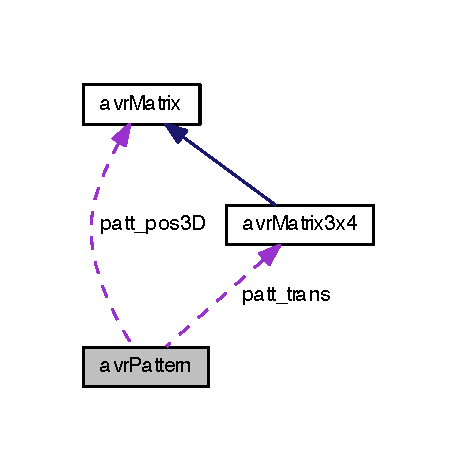
\includegraphics[width=219pt]{classavr_pattern__coll__graph}
\end{center}
\end{figure}
\subsection*{Public Member Functions}
\begin{DoxyCompactItemize}
\item 
\hypertarget{classavr_pattern_a05f2998048e17c4c0c9aad6f602f11b1}{{\bfseries avr\-Pattern} (const char $\ast$filename, double patt\-\_\-width, double $\ast$patt\-\_\-center=N\-U\-L\-L)}\label{classavr_pattern_a05f2998048e17c4c0c9aad6f602f11b1}

\item 
\hypertarget{classavr_pattern_acbc53b3ae2caa39e890db118045e09f2}{\hyperlink{classavr_matrix3x4}{avr\-Matrix3x4} \& {\bfseries trans} ()}\label{classavr_pattern_acbc53b3ae2caa39e890db118045e09f2}

\item 
\hypertarget{classavr_pattern_affbc11f7ae1f22c9a9fefb855bd6e5b4}{\hyperlink{classavr_matrix}{avr\-Matrix} \& {\bfseries pos3\-D} ()}\label{classavr_pattern_affbc11f7ae1f22c9a9fefb855bd6e5b4}

\item 
\hypertarget{classavr_pattern_acfa3004188b0e188856d99e16b845009}{double {\bfseries width} ()}\label{classavr_pattern_acfa3004188b0e188856d99e16b845009}

\item 
\hypertarget{classavr_pattern_a212a6fc4a9acab9ae06a5fcab82b9c0d}{double {\bfseries accuracy} ()}\label{classavr_pattern_a212a6fc4a9acab9ae06a5fcab82b9c0d}

\item 
\hypertarget{classavr_pattern_aead37a67a2a0ff500b071bd9bafa7c15}{double $\ast$ {\bfseries center} ()}\label{classavr_pattern_aead37a67a2a0ff500b071bd9bafa7c15}

\item 
\hypertarget{classavr_pattern_ab038de2d8ebc3633cd5bbd55d18298a1}{std\-::string {\bfseries name} ()}\label{classavr_pattern_ab038de2d8ebc3633cd5bbd55d18298a1}

\item 
\hypertarget{classavr_pattern_afd677bd736475b0975371795a7bb0209}{bool {\bfseries visible} ()}\label{classavr_pattern_afd677bd736475b0975371795a7bb0209}

\item 
\hypertarget{classavr_pattern_a1d5dc06248a365f6acdef536ae783bf5}{int {\bfseries id} ()}\label{classavr_pattern_a1d5dc06248a365f6acdef536ae783bf5}

\item 
\hypertarget{classavr_pattern_a148de7180212abbdfa81431507c40a9b}{void {\bfseries set\-I\-D} (int id)}\label{classavr_pattern_a148de7180212abbdfa81431507c40a9b}

\item 
\hypertarget{classavr_pattern_acd22f88723f72538e1361ec676443c53}{void {\bfseries set\-Name} (std\-::string name)}\label{classavr_pattern_acd22f88723f72538e1361ec676443c53}

\item 
\hypertarget{classavr_pattern_ae77864f7a3e4c247226f87fa0a4b2693}{void {\bfseries set\-Width} (double width)}\label{classavr_pattern_ae77864f7a3e4c247226f87fa0a4b2693}

\item 
\hypertarget{classavr_pattern_a5f2fa1a6320d44764adfbb8c6e074b87}{void {\bfseries set\-Visible} (bool visible)}\label{classavr_pattern_a5f2fa1a6320d44764adfbb8c6e074b87}

\item 
\hypertarget{classavr_pattern_af91b558c29fde6b897821dd48cf82c9f}{void {\bfseries set\-Center} (double center\mbox{[}2\mbox{]})}\label{classavr_pattern_af91b558c29fde6b897821dd48cf82c9f}

\item 
\hypertarget{classavr_pattern_a990cea7c04156ce2fcbe7295bdc0da80}{void {\bfseries set\-Accuracy} (double accuracy)}\label{classavr_pattern_a990cea7c04156ce2fcbe7295bdc0da80}

\end{DoxyCompactItemize}
\subsection*{Static Public Member Functions}
\begin{DoxyCompactItemize}
\item 
static \hyperlink{classavr_pattern}{avr\-Pattern} $\ast$ \hyperlink{classavr_pattern_aa18165a5bf930e986f3f5051e29c26d9}{avr\-Read\-Config\-File\-Not\-Relation} (const char $\ast$filename, int $\ast$number\-Patts)
\begin{DoxyCompactList}\small\item\em auxiliary function, reads the config file of the markers W\-I\-T\-H\-O\-U\-T relation between them pre-\/calculated \end{DoxyCompactList}\item 
static \hyperlink{classavr_pattern}{avr\-Pattern} $\ast$ \hyperlink{classavr_pattern_a5be573c62e61d14544fe68f9af5f2a95}{avr\-Read\-Config\-File\-With\-Relation} (const char $\ast$filename, int $\ast$number\-Patts)
\begin{DoxyCompactList}\small\item\em auxiliary function, reads the config file of the markers W\-I\-T\-H relation between them pre-\/calculated \end{DoxyCompactList}\end{DoxyCompactItemize}
\subsection*{Protected Attributes}
\begin{DoxyCompactItemize}
\item 
\hypertarget{classavr_pattern_a616c3c9504c49b4c454612a983652312}{\hyperlink{classavr_matrix}{avr\-Matrix} $\ast$ {\bfseries patt\-\_\-pos3\-D}}\label{classavr_pattern_a616c3c9504c49b4c454612a983652312}

\item 
\hypertarget{classavr_pattern_a71ba1b6c2e055212af6b053ad2f30f90}{\hyperlink{classavr_matrix3x4}{avr\-Matrix3x4} $\ast$ {\bfseries patt\-\_\-trans}}\label{classavr_pattern_a71ba1b6c2e055212af6b053ad2f30f90}

\end{DoxyCompactItemize}


\subsection{Detailed Description}
This class stores all information of a marker pattern which was registered in the application. 

Stored Informations\par
 \begin{DoxyItemize}
\item identifier \item visibility state \item name (opcional) \item real width of the marker (in millimeters) \item accuracy \item center coordinates \item final position matrix (internal use) \item transformation matrix\end{DoxyItemize}

\begin{DoxyParams}{Parameters}
{\em filename} & path of the file that defines the marker pattern \\
\hline
{\em patt\-\_\-width} & real width of the marker (in millimeters) \\
\hline
{\em patt\-\_\-center} & center coordinates of the marker \\
\hline
\end{DoxyParams}


\subsection{Member Function Documentation}
\hypertarget{classavr_pattern_aa18165a5bf930e986f3f5051e29c26d9}{\index{avr\-Pattern@{avr\-Pattern}!avr\-Read\-Config\-File\-Not\-Relation@{avr\-Read\-Config\-File\-Not\-Relation}}
\index{avr\-Read\-Config\-File\-Not\-Relation@{avr\-Read\-Config\-File\-Not\-Relation}!avrPattern@{avr\-Pattern}}
\subsubsection[{avr\-Read\-Config\-File\-Not\-Relation}]{\setlength{\rightskip}{0pt plus 5cm}static {\bf avr\-Pattern}$\ast$ avr\-Pattern\-::avr\-Read\-Config\-File\-Not\-Relation (
\begin{DoxyParamCaption}
\item[{const char $\ast$}]{filename, }
\item[{int $\ast$}]{number\-Patts}
\end{DoxyParamCaption}
)\hspace{0.3cm}{\ttfamily [static]}}}\label{classavr_pattern_aa18165a5bf930e986f3f5051e29c26d9}


auxiliary function, reads the config file of the markers W\-I\-T\-H\-O\-U\-T relation between them pre-\/calculated 


\begin{DoxyParams}[1]{Parameters}
\mbox{\tt in}  & {\em filename} & config file path \\
\hline
\mbox{\tt out}  & {\em number\-Patts} & number of markers registered \\
\hline
\end{DoxyParams}
\begin{DoxyReturn}{Returns}
avr\-Pattern$\ast$ array with the avr\-Patterns registered 
\end{DoxyReturn}
\hypertarget{classavr_pattern_a5be573c62e61d14544fe68f9af5f2a95}{\index{avr\-Pattern@{avr\-Pattern}!avr\-Read\-Config\-File\-With\-Relation@{avr\-Read\-Config\-File\-With\-Relation}}
\index{avr\-Read\-Config\-File\-With\-Relation@{avr\-Read\-Config\-File\-With\-Relation}!avrPattern@{avr\-Pattern}}
\subsubsection[{avr\-Read\-Config\-File\-With\-Relation}]{\setlength{\rightskip}{0pt plus 5cm}static {\bf avr\-Pattern}$\ast$ avr\-Pattern\-::avr\-Read\-Config\-File\-With\-Relation (
\begin{DoxyParamCaption}
\item[{const char $\ast$}]{filename, }
\item[{int $\ast$}]{number\-Patts}
\end{DoxyParamCaption}
)\hspace{0.3cm}{\ttfamily [static]}}}\label{classavr_pattern_a5be573c62e61d14544fe68f9af5f2a95}


auxiliary function, reads the config file of the markers W\-I\-T\-H relation between them pre-\/calculated 


\begin{DoxyParams}[1]{Parameters}
\mbox{\tt in}  & {\em filename} & config file path \\
\hline
\mbox{\tt out}  & {\em number\-Patts} & number of markers registered \\
\hline
\end{DoxyParams}
\begin{DoxyReturn}{Returns}
avr\-Pattern$\ast$ array with the avr\-Patterns registered 
\end{DoxyReturn}


The documentation for this class was generated from the following file\-:\begin{DoxyCompactItemize}
\item 
avr\-Pattern.\-h\end{DoxyCompactItemize}

\hypertarget{classavr_pattern_info}{\section{avr\-Pattern\-Info Class Reference}
\label{classavr_pattern_info}\index{avr\-Pattern\-Info@{avr\-Pattern\-Info}}
}


main structure for detected patterns of the library internal use.  




{\ttfamily \#include \char`\"{}avr\-Pattern\-Info.\-h\char`\"{}}

\subsection*{Public Attributes}
\begin{DoxyCompactItemize}
\item 
\hypertarget{classavr_pattern_info_a3a0093ce9ac05bb2745a1fa682a23438}{int {\bfseries area}}\label{classavr_pattern_info_a3a0093ce9ac05bb2745a1fa682a23438}

\item 
\hypertarget{classavr_pattern_info_af72af1ef28567a03f9c14790e50caba3}{int {\bfseries id}}\label{classavr_pattern_info_af72af1ef28567a03f9c14790e50caba3}

\item 
\hypertarget{classavr_pattern_info_a1dd7c2ee70ebee15851798a6e140d2aa}{int {\bfseries dir}}\label{classavr_pattern_info_a1dd7c2ee70ebee15851798a6e140d2aa}

\item 
\hypertarget{classavr_pattern_info_a3890f6ae1571597f3ce6a18ce88f07a5}{double {\bfseries cf}}\label{classavr_pattern_info_a3890f6ae1571597f3ce6a18ce88f07a5}

\item 
\hypertarget{classavr_pattern_info_a9a6b2c6270b15d0df992c1b97eb1ebd9}{double {\bfseries pos} \mbox{[}2\mbox{]}}\label{classavr_pattern_info_a9a6b2c6270b15d0df992c1b97eb1ebd9}

\item 
\hypertarget{classavr_pattern_info_a877d45bbae69bc4a70fcd83fed56c316}{double {\bfseries line} \mbox{[}4\mbox{]}\mbox{[}3\mbox{]}}\label{classavr_pattern_info_a877d45bbae69bc4a70fcd83fed56c316}

\item 
\hypertarget{classavr_pattern_info_a81b663e52fb6304d7a8803ba1149d2f8}{double {\bfseries vertex} \mbox{[}4\mbox{]}\mbox{[}2\mbox{]}}\label{classavr_pattern_info_a81b663e52fb6304d7a8803ba1149d2f8}

\end{DoxyCompactItemize}


\subsection{Detailed Description}
main structure for detected patterns of the library internal use. 

Store information after contour detection (in ideal screen coordinate, after distortion compensated). \begin{DoxyNote}{Note}
Lines are represented by 3 values a,b,c for ax+by+c=0 
\end{DoxyNote}


The documentation for this class was generated from the following file\-:\begin{DoxyCompactItemize}
\item 
avr\-Pattern\-Info.\-h\end{DoxyCompactItemize}

\hypertarget{classavr_system_auto_multi}{\section{avr\-System\-Auto\-Multi Class Reference}
\label{classavr_system_auto_multi}\index{avr\-System\-Auto\-Multi@{avr\-System\-Auto\-Multi}}
}


manages marker patterns with relations between them (calculated in real time)  




{\ttfamily \#include \char`\"{}avr\-System\-Auto\-Multi.\-h\char`\"{}}



Inheritance diagram for avr\-System\-Auto\-Multi\-:\nopagebreak
\begin{figure}[H]
\begin{center}
\leavevmode
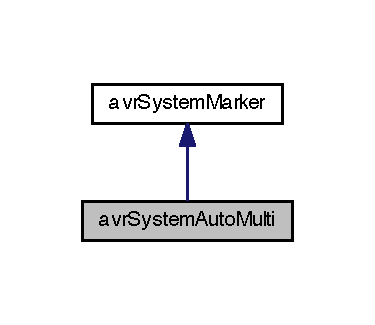
\includegraphics[width=180pt]{classavr_system_auto_multi__inherit__graph}
\end{center}
\end{figure}


Collaboration diagram for avr\-System\-Auto\-Multi\-:\nopagebreak
\begin{figure}[H]
\begin{center}
\leavevmode
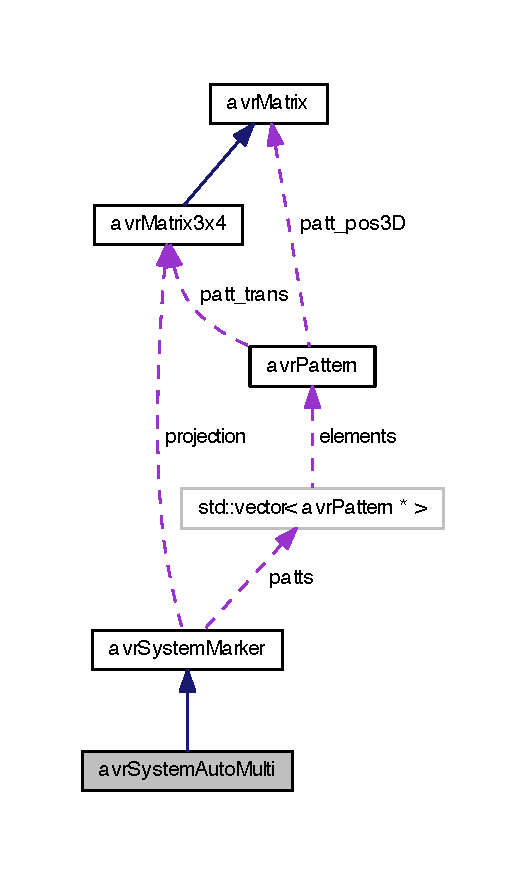
\includegraphics[width=253pt]{classavr_system_auto_multi__coll__graph}
\end{center}
\end{figure}
\subsection*{Public Member Functions}
\begin{DoxyCompactItemize}
\item 
\hypertarget{classavr_system_auto_multi_afa47f7680288a953c3b5b7d498efcc1e}{{\bfseries avr\-System\-Auto\-Multi} (int holder\-Mode=M\-O\-D\-E\-\_\-\-N\-E\-A\-R\-\_\-\-P\-R\-O\-J\-E\-C\-T\-I\-O\-N, void($\ast$display\-Func)(void)=N\-U\-L\-L)}\label{classavr_system_auto_multi_afa47f7680288a953c3b5b7d498efcc1e}

\item 
\hypertarget{classavr_system_auto_multi_a256dadb3e285a837032df13c1d28b972}{{\bfseries avr\-System\-Auto\-Multi} (int holder\-Mode=M\-O\-D\-E\-\_\-\-N\-E\-A\-R\-\_\-\-P\-R\-O\-J\-E\-C\-T\-I\-O\-N, void($\ast$display\-Func)(int)=N\-U\-L\-L)}\label{classavr_system_auto_multi_a256dadb3e285a837032df13c1d28b972}

\item 
\hypertarget{classavr_system_auto_multi_a99b5740990d70eb05961ee83a54f58f1}{void \hyperlink{classavr_system_auto_multi_a99b5740990d70eb05961ee83a54f58f1}{set\-Main\-Marker} (int main\-Marker)}\label{classavr_system_auto_multi_a99b5740990d70eb05961ee83a54f58f1}

\begin{DoxyCompactList}\small\item\em sets marker responsible by projection \end{DoxyCompactList}\item 
\hypertarget{classavr_system_auto_multi_a723717d68b81968cfe8d654f096383af}{void \hyperlink{classavr_system_auto_multi_a723717d68b81968cfe8d654f096383af}{init\-Pointers} ()}\label{classavr_system_auto_multi_a723717d68b81968cfe8d654f096383af}

\begin{DoxyCompactList}\small\item\em initializes tranf, accuracy\-Tranf and prev\-Tranf \end{DoxyCompactList}\item 
\hypertarget{classavr_system_auto_multi_a5505ab405750f53d912b5bb529aebe07}{int {\bfseries get\-Main\-Marker} ()}\label{classavr_system_auto_multi_a5505ab405750f53d912b5bb529aebe07}

\item 
\hypertarget{classavr_system_auto_multi_a026bfb4ca356b64cf9415a6035335251}{int {\bfseries get\-Holder\-Marker} ()}\label{classavr_system_auto_multi_a026bfb4ca356b64cf9415a6035335251}

\item 
\hypertarget{classavr_system_auto_multi_ab3776d9d3a377e1f8ee130f5b427f641}{\hyperlink{classavr_matrix3x4}{avr\-Matrix3x4} $\ast$ {\bfseries get\-Prev\-Transf} ()}\label{classavr_system_auto_multi_ab3776d9d3a377e1f8ee130f5b427f641}

\item 
\hypertarget{classavr_system_auto_multi_a2120f522f8f9a9d02031db03c37bd925}{\hyperlink{classavr_matrix3x4}{avr\-Matrix3x4} $\ast$ {\bfseries get\-Transf} ()}\label{classavr_system_auto_multi_a2120f522f8f9a9d02031db03c37bd925}

\item 
\hypertarget{classavr_system_auto_multi_aa5fda68ead553d6146ef38f53d12a4ed}{virtual bool \hyperlink{classavr_system_auto_multi_aa5fda68ead553d6146ef38f53d12a4ed}{set\-Camera\-Transformation} (\hyperlink{classavr_pattern_info}{avr\-Pattern\-Info} $\ast$marker\-\_\-info, int marker\-\_\-num)}\label{classavr_system_auto_multi_aa5fda68ead553d6146ef38f53d12a4ed}

\begin{DoxyCompactList}\small\item\em calculates the camera transfomation relative the each marker pattern \end{DoxyCompactList}\item 
\hypertarget{classavr_system_auto_multi_a8fc6be5311998a51056f8f4b2e443094}{virtual void \hyperlink{classavr_system_auto_multi_a8fc6be5311998a51056f8f4b2e443094}{set\-Object\-Transformation} ()}\label{classavr_system_auto_multi_a8fc6be5311998a51056f8f4b2e443094}

\begin{DoxyCompactList}\small\item\em sets object transformation and prepares draw \end{DoxyCompactList}\item 
\hypertarget{classavr_system_auto_multi_a4b34ac9e730e6942e82f3f17a5dd0bb6}{virtual void \hyperlink{classavr_system_auto_multi_a4b34ac9e730e6942e82f3f17a5dd0bb6}{set\-Display\-Callback} (void($\ast$display\-Func)(void))}\label{classavr_system_auto_multi_a4b34ac9e730e6942e82f3f17a5dd0bb6}

\begin{DoxyCompactList}\small\item\em sets secondary display function \end{DoxyCompactList}\item 
\hypertarget{classavr_system_auto_multi_adb5f93027373d9f360e2e8d20e1b1549}{virtual void \hyperlink{classavr_system_auto_multi_adb5f93027373d9f360e2e8d20e1b1549}{set\-Display\-Callback} (void($\ast$display\-Func)(int))}\label{classavr_system_auto_multi_adb5f93027373d9f360e2e8d20e1b1549}

\begin{DoxyCompactList}\small\item\em sets main display function \end{DoxyCompactList}\item 
\hypertarget{classavr_system_auto_multi_a030a805955fcc90a8082fcb12ad9a80f}{virtual void \hyperlink{classavr_system_auto_multi_a030a805955fcc90a8082fcb12ad9a80f}{draw\-Function} ()}\label{classavr_system_auto_multi_a030a805955fcc90a8082fcb12ad9a80f}

\begin{DoxyCompactList}\small\item\em calls the renderization callback \end{DoxyCompactList}\end{DoxyCompactItemize}
\subsection*{Public Attributes}
\begin{DoxyCompactItemize}
\item 
\hypertarget{classavr_system_auto_multi_a3bd075f84c739fc5778a46e6146b874e}{void($\ast$ \hyperlink{classavr_system_auto_multi_a3bd075f84c739fc5778a46e6146b874e}{draw\-Func} )(int id\-Holder)}\label{classavr_system_auto_multi_a3bd075f84c739fc5778a46e6146b874e}

\begin{DoxyCompactList}\small\item\em main display callback \end{DoxyCompactList}\item 
\hypertarget{classavr_system_auto_multi_a374678038af70f4436d7f45947d3cb76}{void($\ast$ \hyperlink{classavr_system_auto_multi_a374678038af70f4436d7f45947d3cb76}{draw\-Func2} )(void)}\label{classavr_system_auto_multi_a374678038af70f4436d7f45947d3cb76}

\begin{DoxyCompactList}\small\item\em secondary display callback \end{DoxyCompactList}\end{DoxyCompactItemize}
\subsection*{Additional Inherited Members}


\subsection{Detailed Description}
manages marker patterns with relations between them (calculated in real time) 


\begin{DoxyParams}{Parameters}
{\em holder\-Mode} & definition mode of the base marker (responsible by renderization) \mbox{[}default is M\-O\-D\-E\-\_\-\-N\-E\-A\-R\-\_\-\-P\-R\-O\-J\-E\-C\-T\-I\-O\-N\mbox{]} Possible modes are\-:\par
 \begin{DoxyItemize}
\item M\-O\-D\-E\-\_\-\-N\-E\-A\-R\-\_\-\-P\-R\-O\-J\-E\-C\-T\-I\-O\-N base marker is the marker most near of the object projected\par
 \item M\-O\-D\-E\-\_\-\-N\-E\-A\-R\-\_\-\-C\-A\-M\-E\-R\-A base marker is the marker most near of the real camera\par
 \item M\-O\-D\-E\-\_\-\-R\-E\-S\-I\-S\-T\-E\-N\-C\-E base marker is the marker which has less state change\par
 \item M\-O\-D\-E\-\_\-\-I\-N\-C\-L\-I\-N\-A\-T\-I\-O\-N base marker is the marker that is less inclined in relation to real camera\par
 \item M\-O\-D\-E\-\_\-\-A\-C\-C\-U\-R\-A\-C\-Y base marker is the marker that has the larger accuracy\par
 \item M\-O\-D\-E\-\_\-\-P\-R\-I\-O\-R\-I\-T\-Y base marker is the first visible marker (in the order of insertion, in other words, in the order shown in the config file) \end{DoxyItemize}
\\
\hline
{\em display} & renderization callback \\
\hline
\end{DoxyParams}


The documentation for this class was generated from the following file\-:\begin{DoxyCompactItemize}
\item 
avr\-System\-Auto\-Multi.\-h\end{DoxyCompactItemize}

\hypertarget{classavr_system_marker}{\section{avr\-System\-Marker Class Reference}
\label{classavr_system_marker}\index{avr\-System\-Marker@{avr\-System\-Marker}}
}


Abstract class for manages the systems marker of the application.  




{\ttfamily \#include \char`\"{}avr\-System\-Marker.\-h\char`\"{}}



Inheritance diagram for avr\-System\-Marker\-:\nopagebreak
\begin{figure}[H]
\begin{center}
\leavevmode
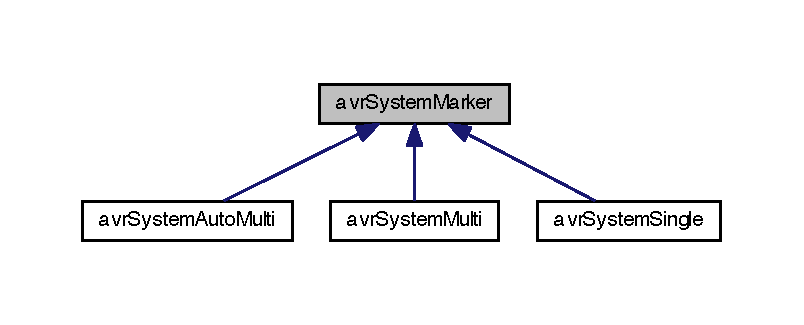
\includegraphics[width=350pt]{classavr_system_marker__inherit__graph}
\end{center}
\end{figure}


Collaboration diagram for avr\-System\-Marker\-:\nopagebreak
\begin{figure}[H]
\begin{center}
\leavevmode
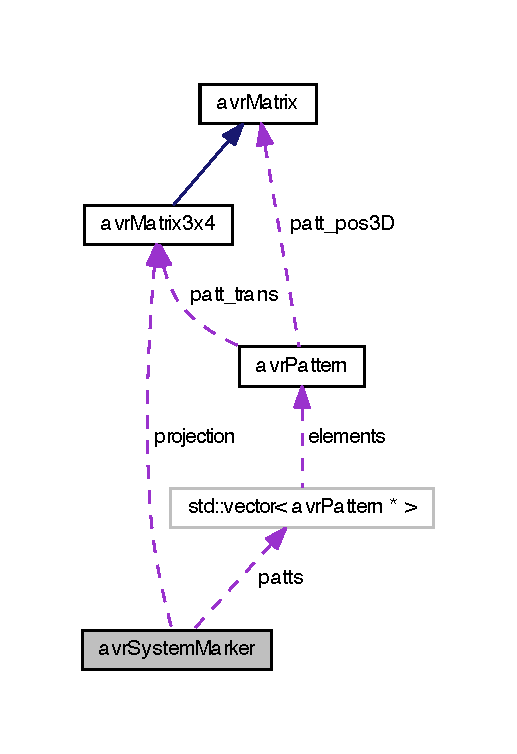
\includegraphics[width=248pt]{classavr_system_marker__coll__graph}
\end{center}
\end{figure}
\subsection*{Public Member Functions}
\begin{DoxyCompactItemize}
\item 
void \hyperlink{classavr_system_marker_ada81a1258d8718041130f8256f127b82}{add\-Pattern} (\hyperlink{classavr_pattern}{avr\-Pattern} \&patt)
\begin{DoxyCompactList}\small\item\em adds marker patterns to the system \end{DoxyCompactList}\item 
\hypertarget{classavr_system_marker_a8bd7531b62e628f53aca79934cc3cbe4}{int \hyperlink{classavr_system_marker_a8bd7531b62e628f53aca79934cc3cbe4}{size\-Patts} () const }\label{classavr_system_marker_a8bd7531b62e628f53aca79934cc3cbe4}

\begin{DoxyCompactList}\small\item\em returns the marker patterns number which aggregate the system \end{DoxyCompactList}\item 
\hypertarget{classavr_system_marker_aca0f590142ff9d881d9d38b085b8eb0a}{\hyperlink{classavr_pattern}{avr\-Pattern} \& \hyperlink{classavr_system_marker_aca0f590142ff9d881d9d38b085b8eb0a}{get\-Patt} (int index) const }\label{classavr_system_marker_aca0f590142ff9d881d9d38b085b8eb0a}

\begin{DoxyCompactList}\small\item\em returns the marker pattern located in position 'index' of the patts vector \end{DoxyCompactList}\item 
\hypertarget{classavr_system_marker_a4169a0baae2d3574818b8ce1f5e5f613}{\hyperlink{classavr_matrix3x4}{avr\-Matrix3x4} \& \hyperlink{classavr_system_marker_a4169a0baae2d3574818b8ce1f5e5f613}{get\-Projection} () const }\label{classavr_system_marker_a4169a0baae2d3574818b8ce1f5e5f613}

\begin{DoxyCompactList}\small\item\em Get the projection matrix. \end{DoxyCompactList}\item 
virtual bool \hyperlink{classavr_system_marker_a565106c7110c5ffd5e9448d4b4349659}{set\-Camera\-Transformation} (\hyperlink{classavr_pattern_info}{avr\-Pattern\-Info} $\ast$marker\-\_\-info, int marker\-\_\-num)=0
\begin{DoxyCompactList}\small\item\em internal use function, calculates the camera transfomation relative the each marker pattern \end{DoxyCompactList}\item 
\hypertarget{classavr_system_marker_a7d1e0f3184871cc973a7e0e4ac0cdfa4}{virtual void \hyperlink{classavr_system_marker_a7d1e0f3184871cc973a7e0e4ac0cdfa4}{set\-Object\-Transformation} ()=0}\label{classavr_system_marker_a7d1e0f3184871cc973a7e0e4ac0cdfa4}

\begin{DoxyCompactList}\small\item\em internal use function, sets object transformation and prepares draw \end{DoxyCompactList}\item 
\hypertarget{classavr_system_marker_a5a01bf7952c90ebf4234d86a93c1a261}{virtual void \hyperlink{classavr_system_marker_a5a01bf7952c90ebf4234d86a93c1a261}{set\-Display\-Callback} (void($\ast$display\-Func)(void))=0}\label{classavr_system_marker_a5a01bf7952c90ebf4234d86a93c1a261}

\begin{DoxyCompactList}\small\item\em sets secondary display function \end{DoxyCompactList}\item 
\hypertarget{classavr_system_marker_a89b996f137d45d3cd2f1adfa6cfebc34}{virtual void \hyperlink{classavr_system_marker_a89b996f137d45d3cd2f1adfa6cfebc34}{set\-Display\-Callback} (void($\ast$display\-Func)(int))=0}\label{classavr_system_marker_a89b996f137d45d3cd2f1adfa6cfebc34}

\begin{DoxyCompactList}\small\item\em sets main display function \end{DoxyCompactList}\item 
\hypertarget{classavr_system_marker_ab237ef95b8a5ab8244074e359382674b}{virtual void \hyperlink{classavr_system_marker_ab237ef95b8a5ab8244074e359382674b}{draw\-Function} ()=0}\label{classavr_system_marker_ab237ef95b8a5ab8244074e359382674b}

\begin{DoxyCompactList}\small\item\em internal use function, calls the renderization callback \end{DoxyCompactList}\end{DoxyCompactItemize}
\subsection*{Protected Attributes}
\begin{DoxyCompactItemize}
\item 
\hypertarget{classavr_system_marker_a979bc77ea440bbdf9fe5737164925450}{std\-::vector$<$ \hyperlink{classavr_pattern}{avr\-Pattern} $\ast$ $>$ {\bfseries patts}}\label{classavr_system_marker_a979bc77ea440bbdf9fe5737164925450}

\item 
\hypertarget{classavr_system_marker_a5e7a6a94a0286fc7b60af9e961dc73a7}{\hyperlink{classavr_matrix3x4}{avr\-Matrix3x4} $\ast$ {\bfseries projection}}\label{classavr_system_marker_a5e7a6a94a0286fc7b60af9e961dc73a7}

\end{DoxyCompactItemize}


\subsection{Detailed Description}
Abstract class for manages the systems marker of the application. 

This class has a vector with the marker patterns registered in the application and the system transformation matrix 

\subsection{Member Function Documentation}
\hypertarget{classavr_system_marker_ada81a1258d8718041130f8256f127b82}{\index{avr\-System\-Marker@{avr\-System\-Marker}!add\-Pattern@{add\-Pattern}}
\index{add\-Pattern@{add\-Pattern}!avrSystemMarker@{avr\-System\-Marker}}
\subsubsection[{add\-Pattern}]{\setlength{\rightskip}{0pt plus 5cm}void avr\-System\-Marker\-::add\-Pattern (
\begin{DoxyParamCaption}
\item[{{\bf avr\-Pattern} \&}]{patt}
\end{DoxyParamCaption}
)}}\label{classavr_system_marker_ada81a1258d8718041130f8256f127b82}


adds marker patterns to the system 


\begin{DoxyParams}[1]{Parameters}
\mbox{\tt in}  & {\em patt} & new marker pattern \\
\hline
\end{DoxyParams}
\begin{DoxyReturn}{Returns}
void 
\end{DoxyReturn}
\hypertarget{classavr_system_marker_a565106c7110c5ffd5e9448d4b4349659}{\index{avr\-System\-Marker@{avr\-System\-Marker}!set\-Camera\-Transformation@{set\-Camera\-Transformation}}
\index{set\-Camera\-Transformation@{set\-Camera\-Transformation}!avrSystemMarker@{avr\-System\-Marker}}
\subsubsection[{set\-Camera\-Transformation}]{\setlength{\rightskip}{0pt plus 5cm}virtual bool avr\-System\-Marker\-::set\-Camera\-Transformation (
\begin{DoxyParamCaption}
\item[{{\bf avr\-Pattern\-Info} $\ast$}]{marker\-\_\-info, }
\item[{int}]{marker\-\_\-num}
\end{DoxyParamCaption}
)\hspace{0.3cm}{\ttfamily [pure virtual]}}}\label{classavr_system_marker_a565106c7110c5ffd5e9448d4b4349659}


internal use function, calculates the camera transfomation relative the each marker pattern 


\begin{DoxyParams}[1]{Parameters}
\mbox{\tt in}  & {\em marker\-\_\-info} & possible marker patterns that were identified by the A\-R\-Tool\-Kit \\
\hline
\mbox{\tt in}  & {\em marker\-\_\-num} & number of marker patterns identified \\
\hline
\end{DoxyParams}
\begin{DoxyReturn}{Returns}
bool 
\end{DoxyReturn}


Implemented in \hyperlink{classavr_system_auto_multi_aa5fda68ead553d6146ef38f53d12a4ed}{avr\-System\-Auto\-Multi}, \hyperlink{classavr_system_single_a295e942652e83adac2305ce58fe12bdd}{avr\-System\-Single}, and \hyperlink{classavr_system_multi_a96fe92b1d7cc08dfb4e8f57d7f0c7d17}{avr\-System\-Multi}.



The documentation for this class was generated from the following file\-:\begin{DoxyCompactItemize}
\item 
avr\-System\-Marker.\-h\end{DoxyCompactItemize}

\hypertarget{classavr_system_multi}{\section{avr\-System\-Multi Class Reference}
\label{classavr_system_multi}\index{avr\-System\-Multi@{avr\-System\-Multi}}
}


manages marker patterns with relations between them (calculated in preprocessing)  




{\ttfamily \#include \char`\"{}avr\-System\-Multi.\-h\char`\"{}}



Inheritance diagram for avr\-System\-Multi\-:\nopagebreak
\begin{figure}[H]
\begin{center}
\leavevmode
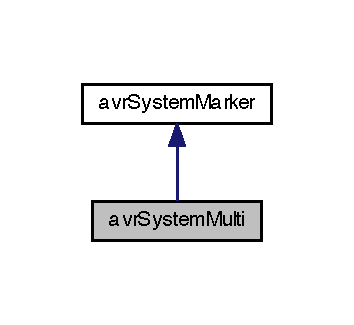
\includegraphics[width=170pt]{classavr_system_multi__inherit__graph}
\end{center}
\end{figure}


Collaboration diagram for avr\-System\-Multi\-:\nopagebreak
\begin{figure}[H]
\begin{center}
\leavevmode
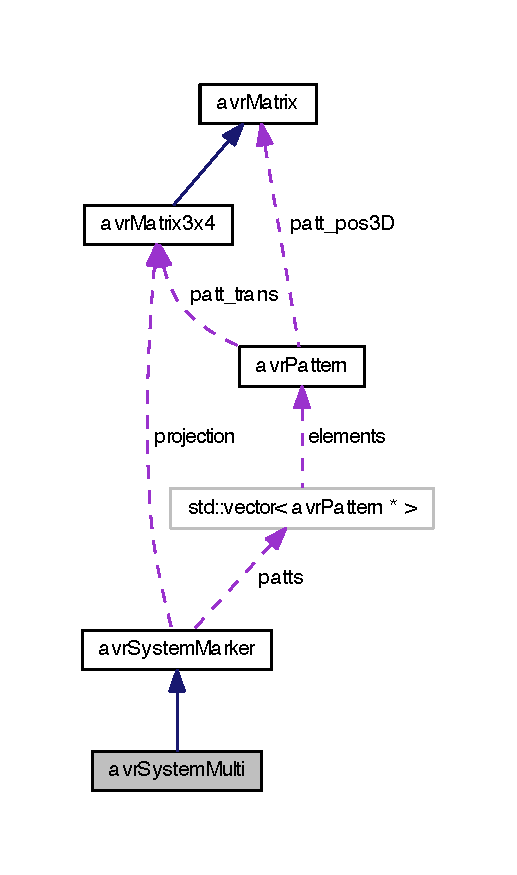
\includegraphics[width=248pt]{classavr_system_multi__coll__graph}
\end{center}
\end{figure}
\subsection*{Public Member Functions}
\begin{DoxyCompactItemize}
\item 
\hypertarget{classavr_system_multi_a5c2395b00dfbcfc5fe8381131997901a}{{\bfseries avr\-System\-Multi} (const char $\ast$filename, void($\ast$display\-Func)(void)=N\-U\-L\-L)}\label{classavr_system_multi_a5c2395b00dfbcfc5fe8381131997901a}

\item 
\hypertarget{classavr_system_multi_aeef640459bbbd037d6d64ce9587c37d6}{{\bfseries avr\-System\-Multi} (const char $\ast$filename, void($\ast$display\-Func)(int)=N\-U\-L\-L)}\label{classavr_system_multi_aeef640459bbbd037d6d64ce9587c37d6}

\item 
\hypertarget{classavr_system_multi_a96fe92b1d7cc08dfb4e8f57d7f0c7d17}{virtual bool \hyperlink{classavr_system_multi_a96fe92b1d7cc08dfb4e8f57d7f0c7d17}{set\-Camera\-Transformation} (\hyperlink{classavr_pattern_info}{avr\-Pattern\-Info} $\ast$marker\-\_\-info, int marker\-\_\-num)}\label{classavr_system_multi_a96fe92b1d7cc08dfb4e8f57d7f0c7d17}

\begin{DoxyCompactList}\small\item\em calculates the camera transfomation relative the each marker pattern \end{DoxyCompactList}\item 
\hypertarget{classavr_system_multi_adeba14fe5306c1c6aad82b2c5103fadf}{virtual void \hyperlink{classavr_system_multi_adeba14fe5306c1c6aad82b2c5103fadf}{set\-Object\-Transformation} ()}\label{classavr_system_multi_adeba14fe5306c1c6aad82b2c5103fadf}

\begin{DoxyCompactList}\small\item\em sets object transformation and prepares draw \end{DoxyCompactList}\item 
\hypertarget{classavr_system_multi_afa378d6fb53f7ee831e1f4acb6214eeb}{virtual void \hyperlink{classavr_system_multi_afa378d6fb53f7ee831e1f4acb6214eeb}{set\-Display\-Callback} (void($\ast$display\-Func)(void))}\label{classavr_system_multi_afa378d6fb53f7ee831e1f4acb6214eeb}

\begin{DoxyCompactList}\small\item\em sets secondary display function \end{DoxyCompactList}\item 
\hypertarget{classavr_system_multi_ae477c6fd28db9f09c98b71def0e5c041}{virtual void \hyperlink{classavr_system_multi_ae477c6fd28db9f09c98b71def0e5c041}{set\-Display\-Callback} (void($\ast$display\-Func)(int))}\label{classavr_system_multi_ae477c6fd28db9f09c98b71def0e5c041}

\begin{DoxyCompactList}\small\item\em sets main display function \end{DoxyCompactList}\item 
\hypertarget{classavr_system_multi_a0c32328ce187e8c040ed7ac0ae10ceeb}{virtual void \hyperlink{classavr_system_multi_a0c32328ce187e8c040ed7ac0ae10ceeb}{draw\-Function} ()}\label{classavr_system_multi_a0c32328ce187e8c040ed7ac0ae10ceeb}

\begin{DoxyCompactList}\small\item\em calls the renderization callback \end{DoxyCompactList}\end{DoxyCompactItemize}
\subsection*{Public Attributes}
\begin{DoxyCompactItemize}
\item 
\hypertarget{classavr_system_multi_afb9a6363fb5550c6a180fa1a42a5d7c1}{void($\ast$ \hyperlink{classavr_system_multi_afb9a6363fb5550c6a180fa1a42a5d7c1}{draw\-Func} )(int id)}\label{classavr_system_multi_afb9a6363fb5550c6a180fa1a42a5d7c1}

\begin{DoxyCompactList}\small\item\em main display callback \end{DoxyCompactList}\item 
\hypertarget{classavr_system_multi_ab1bc1f44dc7b9a3438355ed8a0ef5f65}{void($\ast$ \hyperlink{classavr_system_multi_ab1bc1f44dc7b9a3438355ed8a0ef5f65}{draw\-Func2} )(void)}\label{classavr_system_multi_ab1bc1f44dc7b9a3438355ed8a0ef5f65}

\begin{DoxyCompactList}\small\item\em secondary display callback \end{DoxyCompactList}\end{DoxyCompactItemize}
\subsection*{Additional Inherited Members}


\subsection{Detailed Description}
manages marker patterns with relations between them (calculated in preprocessing) 


\begin{DoxyParams}{Parameters}
{\em filename} & path of the config file of the markers \\
\hline
{\em display} & renderization callback \\
\hline
\end{DoxyParams}


The documentation for this class was generated from the following file\-:\begin{DoxyCompactItemize}
\item 
avr\-System\-Multi.\-h\end{DoxyCompactItemize}

\hypertarget{classavr_system_single}{\section{avr\-System\-Single Class Reference}
\label{classavr_system_single}\index{avr\-System\-Single@{avr\-System\-Single}}
}


manages single marker patterns  




{\ttfamily \#include \char`\"{}avr\-System\-Single.\-h\char`\"{}}



Inheritance diagram for avr\-System\-Single\-:\nopagebreak
\begin{figure}[H]
\begin{center}
\leavevmode
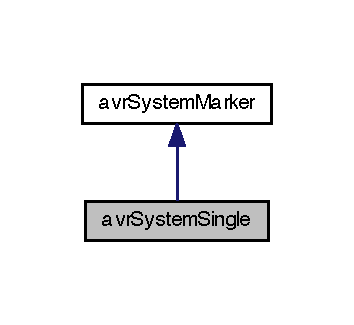
\includegraphics[width=170pt]{classavr_system_single__inherit__graph}
\end{center}
\end{figure}


Collaboration diagram for avr\-System\-Single\-:\nopagebreak
\begin{figure}[H]
\begin{center}
\leavevmode
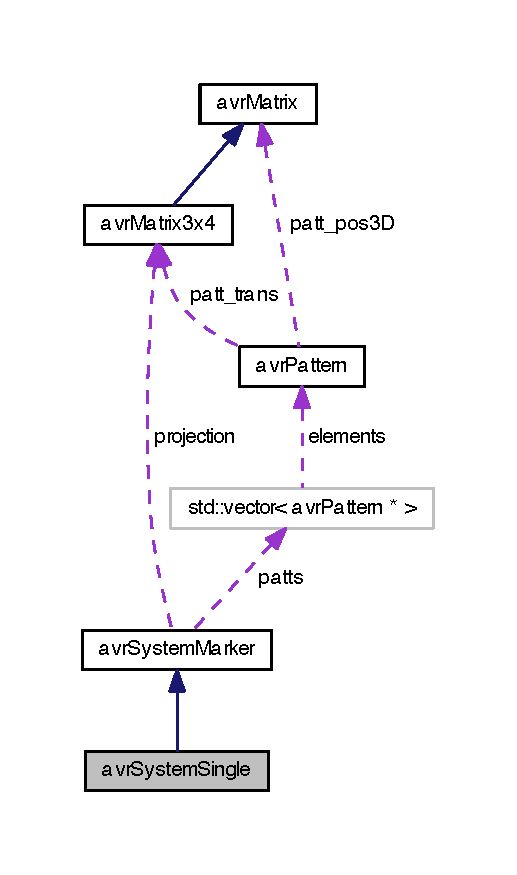
\includegraphics[width=248pt]{classavr_system_single__coll__graph}
\end{center}
\end{figure}
\subsection*{Public Member Functions}
\begin{DoxyCompactItemize}
\item 
\hypertarget{classavr_system_single_a25777b4804b90f0b07bea81bac2a76ea}{{\bfseries avr\-System\-Single} (const char $\ast$filename, double width, double $\ast$center=N\-U\-L\-L, void($\ast$display\-Func)(void)=N\-U\-L\-L)}\label{classavr_system_single_a25777b4804b90f0b07bea81bac2a76ea}

\item 
\hypertarget{classavr_system_single_a3d1e92b11e29b3a512b57c149f75e0ca}{{\bfseries avr\-System\-Single} (const char $\ast$filename, double width, double $\ast$center=N\-U\-L\-L, void($\ast$display\-Func)(int)=N\-U\-L\-L)}\label{classavr_system_single_a3d1e92b11e29b3a512b57c149f75e0ca}

\item 
\hypertarget{classavr_system_single_a295e942652e83adac2305ce58fe12bdd}{virtual bool \hyperlink{classavr_system_single_a295e942652e83adac2305ce58fe12bdd}{set\-Camera\-Transformation} (\hyperlink{classavr_pattern_info}{avr\-Pattern\-Info} $\ast$marker\-\_\-info, int marker\-\_\-num)}\label{classavr_system_single_a295e942652e83adac2305ce58fe12bdd}

\begin{DoxyCompactList}\small\item\em calculates the camera transfomation relative the each marker pattern \end{DoxyCompactList}\item 
\hypertarget{classavr_system_single_a8b87bd9c86e02427ea210eac6ffc45ea}{virtual void \hyperlink{classavr_system_single_a8b87bd9c86e02427ea210eac6ffc45ea}{set\-Object\-Transformation} ()}\label{classavr_system_single_a8b87bd9c86e02427ea210eac6ffc45ea}

\begin{DoxyCompactList}\small\item\em sets object transformation and prepares draw \end{DoxyCompactList}\item 
\hypertarget{classavr_system_single_a796f9552387f638896c154aee433c511}{virtual void \hyperlink{classavr_system_single_a796f9552387f638896c154aee433c511}{set\-Display\-Callback} (void($\ast$display\-Func)(void))}\label{classavr_system_single_a796f9552387f638896c154aee433c511}

\begin{DoxyCompactList}\small\item\em sets secondary display function \end{DoxyCompactList}\item 
\hypertarget{classavr_system_single_a85f602cb791f1e9f6453df363cc1ff6d}{virtual void \hyperlink{classavr_system_single_a85f602cb791f1e9f6453df363cc1ff6d}{set\-Display\-Callback} (void($\ast$display\-Func)(int))}\label{classavr_system_single_a85f602cb791f1e9f6453df363cc1ff6d}

\begin{DoxyCompactList}\small\item\em sets main display function \end{DoxyCompactList}\item 
\hypertarget{classavr_system_single_a6664aa63cfc119ef461de3b24b03bda5}{virtual void \hyperlink{classavr_system_single_a6664aa63cfc119ef461de3b24b03bda5}{draw\-Function} ()}\label{classavr_system_single_a6664aa63cfc119ef461de3b24b03bda5}

\begin{DoxyCompactList}\small\item\em calls the renderization callback \end{DoxyCompactList}\end{DoxyCompactItemize}
\subsection*{Public Attributes}
\begin{DoxyCompactItemize}
\item 
\hypertarget{classavr_system_single_a1b9aa46cfd25de274c7375439ef75339}{void($\ast$ \hyperlink{classavr_system_single_a1b9aa46cfd25de274c7375439ef75339}{draw\-Func} )(int id)}\label{classavr_system_single_a1b9aa46cfd25de274c7375439ef75339}

\begin{DoxyCompactList}\small\item\em main display callback \end{DoxyCompactList}\item 
\hypertarget{classavr_system_single_a7ea216b2e44684e7bec21e8dbdf6f797}{void($\ast$ \hyperlink{classavr_system_single_a7ea216b2e44684e7bec21e8dbdf6f797}{draw\-Func2} )(void)}\label{classavr_system_single_a7ea216b2e44684e7bec21e8dbdf6f797}

\begin{DoxyCompactList}\small\item\em secondary display callback \end{DoxyCompactList}\end{DoxyCompactItemize}
\subsection*{Additional Inherited Members}


\subsection{Detailed Description}
manages single marker patterns 


\begin{DoxyParams}{Parameters}
{\em filename} & path of the file that defines the marker pattern \\
\hline
{\em width} & real width of the marker (in millimeters) \\
\hline
{\em center} & center coordinates of the marker \\
\hline
{\em display} & renderization callback \\
\hline
\end{DoxyParams}


The documentation for this class was generated from the following file\-:\begin{DoxyCompactItemize}
\item 
avr\-System\-Single.\-h\end{DoxyCompactItemize}

%--- End generated contents ---

% Index
\newpage
\phantomsection
\addcontentsline{toc}{part}{Index}
\printindex

\end{document}
